\providecommand{\Fun}{\operatorname{Fun}}
\providecommand{\qcOne}{\mathbf{1}}   %
\providecommand{\qcTwo}{\mathbf{2}}   %
\providecommand{\hciso}{\mathbb{I}}    %
\providecommand{\Rari}{\mathcal{R}ari}     %
\providecommand{\Lari}{\mathcal{L}ari}     %

\section{宇宙论嵌入的∞-宇宙}\label{sec:cosmologically-embedded-cosmoi}

本节将\cref{lem:full-subcategory-cosmos}——它曾被用于证明\trDiscrete{}
\trInfinityCategory{}的子范畴继承一个∞-宇宙结构——推广到\trInfinityCosmos{}的
那些并不全的子范畴。我们将发现，这里有许多有趣的例子。

对任何\trInfinityCosmos{} $\mathcal{K}$ 及其底 1-范畴的任何子范畴——亦即其
对象的一个子集与 0-箭头的一个子范畴——都可以造出一个拟范畴式富集子范畴
$\mathcal{L}\subset\mathcal{K}$，它恰好包含那些对象与 0-箭头以及由它们张成的
一切更高维箭头。我们把这样的子范畴称为\textbf{在正维箭头上为满的}（full on
positive-dimensional arrows）；注意 $\mathcal{L}$ 的诸\trFunctorSpace{}都是%
\trQuasiCategory{}，因为一切内号角包含都在顶点上为双射的。我们对满足进一步
「充盈性」条件的子范畴有特别的兴趣。

\begin{definition}\label{def:replete-subcategory}
设 $\mathcal{K}$ 是一个\trInfinityCosmos{}。子范畴 $\mathcal{L}\subset\mathcal{K}$
称为在 $\mathcal{K}$ 中\textbf{充盈}的，如果它在正维箭头上为满，而且：
\begin{itemize}
\item[(i)] $\mathcal{K}$ 中每个与 $\mathcal{L}$ 中某个对象\trEquivalence{}的%
\trInfinityCategory{}都落在 $\mathcal{L}$ 中。
\item[(ii)] $\mathcal{K}$ 中 $\mathcal{L}$ 的诸对象之间的任何\trEquivalence{}%
都落在 $\mathcal{L}$ 中。
\item[(iii)] $\mathcal{K}$ 中在 $\mathcal{K}$ 内同构于 $\mathcal{L}$ 中某支
0-箭头的任何 0-箭头都落在 $\mathcal{L}$ 中。
\end{itemize}
\end{definition}

\trInfinityCosmos{}的充盈子范畴之包含既是一个\trMonomorphism{}，也是一个
$(\infty,2)$-范畴意义下的\trIsofibration{}，其确切含义见
\cref{ex:replete-local-isofibration}。

\begin{lemma}\label{lem:replete-representable-isofibration}
设 $\mathcal{L}\subset\mathcal{K}$ 是某个\trInfinityCosmos{}的一个充盈子范畴。
那么 $\mathcal{L}$ 中定义出 $\mathcal{K}$ 中\trIsofibration{}的任何映射
$p\colon E\to B$ 都是 $\mathcal{L}$ 中可表示地定义的\trIsofibration{}：也就是
说，对所有 $X\in\mathcal{L}$，映射
$p_{*}\colon\Fun_{\mathcal{L}}(X,E)\twoheadrightarrow\Fun_{\mathcal{L}}(X,B)$
是\trQuasiCategory{}之间的\trIsofibration{}。
\end{lemma}

\begin{proof}
由于 $\mathcal{K}$ 是一个\trInfinityCosmos{}，等价纤维化公理
\cref{def:infinity-cosmos}(ii) 要求
$p_{*}\colon\Fun_{\mathcal{K}}(X,E)\twoheadrightarrow\Fun_{\mathcal{K}}(X,B)$
是\trQuasiCategory{}之间的\trIsofibration{}。由于内号角包含都在顶点上为双射
的，而 $\Fun_{\mathcal{L}}(X,E)\hookrightarrow\Fun_{\mathcal{K}}(X,E)$ 在正维
箭头上为满，限制后的映射
$p_{*}\colon\Fun_{\mathcal{L}}(X,E)\twoheadrightarrow\Fun_{\mathcal{L}}(X,B)$
立即对内号角包含具有提升性质。于是只剩下求解下左图所示形状的提升问题
\begin{center}
\begin{tikzpicture}[x=1.5em,y=1.5em]
  \node (tl) at (0,1.7) {$\qcOne$};
  \node (tm) at (4.8,1.7) {$\Fun_{\mathcal{L}}(X,E)$};
  \node (tr) at (11.2,1.7) {$\Fun_{\mathcal{K}}(X,E)$};
  \node (bl) at (0,-1.7) {$\hciso$};
  \node (bm) at (4.8,-1.7) {$\Fun_{\mathcal{L}}(X,B)$};
  \node (br) at (11.2,-1.7) {$\Fun_{\mathcal{K}}(X,B)$};
  \draw[->] (0.6,1.7) -- node[above]{$\scriptstyle e$} (3.0,1.7);
  \draw[right hook->] (6.9,1.7) -- (9.2,1.7);
  \draw[right hook->] (0,1.15) -- (0,-1.15);
  \draw[->] (0.6,-1.7) -- node[below]{$\scriptstyle\beta$} (3.0,-1.7);
  \draw[right hook->] (6.9,-1.7) -- (9.2,-1.7);
  \draw[->] (7.4,1.15) -- node[right]{$\scriptstyle p_{*}$} (7.4,-1.15);
  \draw[->] (11.2,1.15) -- node[right]{$\scriptstyle p_{*}$} (11.2,-1.15);
  \draw[->,dotted] (0.75,-1.3) -- (3.5,1.35);
  \draw[->,dashed] (5.8,-1.4) -- (10.0,1.35);
\end{tikzpicture}
\end{center}
该提升问题定义了 $\mathcal{L}$ 中一支 0-箭头 $e\colon X\to E$ 与 $\mathcal{L}$
中一个\trHomotopyCoherentIsomorphism{} $\beta\colon b\cong pe$。它在 $\mathcal{K}$
中的解定义了 $\mathcal{K}$ 中一支 0-箭头 $e'\colon X\to E$ 使得 $pe'=b$，并
配有 $\mathcal{K}$ 中一个\trHomotopyCoherentIsomorphism{} $e\cong e'$。由在
正维箭头上的满性，为证此提升经由包含
$\Fun_{\mathcal{L}}(X,E)\hookrightarrow\Fun_{\mathcal{K}}(X,E)$ 分解，只需论证
映射 $e'$ 落在 $\mathcal{L}$ 中，而由\cref{def:replete-subcategory}(iii) 情形
正是如此。
\end{proof}

下面的结果描述了一个条件，使得充盈子范畴 $\mathcal{L}\subset\mathcal{K}$ 在此
条件下继承一个从 $\mathcal{K}$ 创生的∞-宇宙结构。

\begin{proposition}\label{prop:cosmologically-embedded}
设 $\mathcal{L}\subset\mathcal{K}$ 是某个\trInfinityCosmos{}的一个充盈子范畴。
若 $\mathcal{L}$ 在 $\mathcal{K}$ 中对\trFlexibleWeightedLimit{}封闭，则
$\mathcal{L}$ 定义出一个∞-宇宙，其等价纤维化、等价、平凡纤维化与单纯极限均由
包含 $\mathcal{L}\hookrightarrow\mathcal{K}$ 创生，从而该包含定义一个%
\trCosmologicalFunctor{}。
\end{proposition}

当这些条件成立时，我们把 $\mathcal{L}$ 称为 $\mathcal{K}$ 的一个\textbf{%
\trCosmologicalEmbedding{}的\trInfinityCosmos}（cosmologically embedded
∞-cosmos），把 $\mathcal{L}\hookrightarrow\mathcal{K}$ 称为一个\textbf{%
\trCosmologicalEmbedding}（cosmological embedding）。这一术语既反映了充盈子
范畴包含的嵌入性质，也反映了其类等价纤维化的性质。

\begin{proof}
说充盈子范畴 $\mathcal{L}\hookrightarrow\mathcal{K}$ 对%
\trFlexibleWeightedLimit{}封闭，意思是：对 $\mathcal{L}$ 中的任何\trDiagram{}%
与 $\mathcal{K}$ 中该图表之上的任何极限锥，此极限锥都落在 $\mathcal{L}$ 中，
并且在子范畴 $\mathcal{L}$ 中满足定义 A.6.5 相应的单纯富集\trUniversalProperty{}。
我们必须验证公理 \cref{def:infinity-cosmos}(i) 的每一种\trLimit{}都在
$\mathcal{L}$ 中存在。立即可得：$\mathcal{L}$ 拥有终对象、\trProduct{}与单纯%
\trCotensor{}，因为这些都属于\trFlexibleWeightedLimit{}，且每一种极限都从
$\mathcal{K}$ 继承而来。由\cref{lem:iso-commas-flexible}与\ref{lem:iso-towers-flexible}，
$\mathcal{L}$ 也容许同构逗号对象与同构塔的构造，同样在 $\mathcal{K}$ 中形成。

将 $\mathcal{L}$ 中的等价纤维化类定义为 $\mathcal{L}$ 中那些在 $\mathcal{K}$ 中
定义等价纤维化的映射。由\cref{lem:iso-commas-pullbacks}与\ref{lem:iso-towers-inverse-limits}，
\trIsofibration{}的\trPullback{}与塔之极限在 $\mathcal{K}$ 中等价于在同一批图表上形成
的同构逗号与同构塔。既然后者这些极限锥按假设落在 $\mathcal{L}$ 中，那么由
$\mathcal{L}$ 在 $\mathcal{K}$ 中的充盈性，与之等价的前者也落在 $\mathcal{L}$ 中。

还有一点尚待验证：即\trIsofibration{}的\trPullback{}与塔之极限在 $\mathcal{L}$ 中作为
锥形\trLimit{}满足单纯富集\trUniversalProperty{}。就 $\mathcal{L}$ 中的\trPullback{}图表
\begin{center}
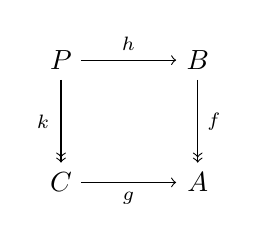
\begin{tikzpicture}[x=1.3em,y=1.3em]
  \node (P) at (0,1.7) {$P$};
  \node (B) at (3.8,1.7) {$B$};
  \node (C) at (0,-1.7) {$C$};
  \node (A) at (3.8,-1.7) {$A$};
  \draw[->] (0.55,1.7) -- node[above]{$\scriptstyle h$} (3.2,1.7);
  \draw[->>] (0,1.15) -- (0,-1.15);
  \node at (0.5,0.6) {$\scriptstyle\lrcorner$};
  \node at (-0.5,0) {$\scriptstyle k$};
  \draw[->>] (3.8,1.15) -- node[right]{$\scriptstyle f$} (3.8,-1.15);
  \draw[->] (0.55,-1.7) -- node[below]{$\scriptstyle g$} (3.2,-1.7);
\end{tikzpicture}
\end{center}
而言，我们必须证明：对每个 $X\in\mathcal{L}$，\trFunctorSpace{}
$\Fun_{\mathcal{L}}(X,P)$ 同构于\trFunctorSpace{}的\trPullback{}
$\Fun_{\mathcal{L}}(X,C)\times_{\Fun_{\mathcal{L}}(X,A)}\Fun_{\mathcal{L}}(X,B)$。

在 $\mathcal{K}$ 中，诸\trFunctorSpace{}之间有这样一张同构，而且鉴于交换图表
\begin{center}
\begin{tikzpicture}[x=1.5em,y=1.5em]
  \node (tl) at (0,1.6) {$\Fun_{\mathcal{L}}(X,P)$};
  \node (tr) at (9.6,1.6)
    {$\Fun_{\mathcal{L}}(X,C)\times_{\Fun_{\mathcal{L}}(X,A)}\Fun_{\mathcal{L}}(X,B)$};
  \node (bl) at (0,-1.6) {$\Fun_{\mathcal{K}}(X,P)$};
  \node (br) at (9.6,-1.6)
    {$\Fun_{\mathcal{K}}(X,C)\times_{\Fun_{\mathcal{K}}(X,A)}\Fun_{\mathcal{K}}(X,B)$};
  \draw[->,dotted] (2.0,1.6) -- (4.6,1.6);
  \draw[right hook->] (0,1.0) -- (0,-1.0);
  \draw[right hook->] (9.6,1.0) -- (9.6,-1.0);
  \draw[->] (2.4,-1.6) -- node[below]{$\scriptstyle\cong$} (5.4,-1.6);
\end{tikzpicture}
\end{center}
以及在正维箭头上的满性，我们只需验证这张点线映射在 0-箭头上的满射性。于是
考虑 $\mathcal{L}$ 中该\trPullback{}图表之上的一个锥（$b\colon X\to B$，$c\colon X\to C$）。
由同构逗号对象 $C\times^{\hciso}_{A}B$ 的\trUniversalProperty{}，存在 $\mathcal{L}$
中的一个因子分解 $\gamma\colon X\to C\times^{\hciso}_{A}B$。与\trEquivalence{}
$C\times^{\hciso}_{A}B\simeq P$ 复合后，这个映射等价于锥 $(b,c)$ 穿过 $\mathcal{K}$
中极限锥 $(h,k)$ 的因子分解 $z\colon X\to P$——后者之所以存在，是因为\trPullback{}在
那里拥有严格\trUniversalProperty{}。由充盈性，$z$ 与「$\gamma$ 同该\trEquivalence{}%
之复合」之间的同构已足以说明 $z$ 落在 $\mathcal{L}$ 中。因此，$\mathcal{L}$ 中的
诸\trFunctorSpace{}同构。一个援引\cref{lem:iso-towers-inverse-limits}的类似
论证证明：\trIsofibration{}之塔的逆向极限在 $\mathcal{L}$ 中定义锥形\trLimit{}。
这就完成了对极限公理 \cref{def:infinity-cosmos}(i) 的证明。

由于 $\mathcal{L}$ 中的诸\trIsofibration{}是 $\mathcal{K}$ 中诸%
\trIsofibration{}的一个子集，而且两种语境下的极限构造相互重合，
\cref{def:infinity-cosmos}(ii) 的诸闭合性质大多从 $\mathcal{K}$ 中的闭合性质
继承而来。唯一的例外是「$\mathcal{L}$ 中的诸\trIsofibration{}可表示地定义%
\trQuasiCategory{}之间的\trIsofibration」这一要求，而这对任何充盈子范畴都已
在\cref{lem:replete-representable-isofibration}中证明。这就证明了 $\mathcal{L}$
定义一个∞-宇宙。

最后，我们论证 $\mathcal{L}$ 中的诸\trEquivalence{}由 $\mathcal{K}$ 的诸%
\trEquivalence{}创生，从而也将推出 $\mathcal{L}$ 中的诸\trTrivialFibration{}%
与 $\mathcal{K}$ 的相重合。\cref{def:replete-subcategory}(ii) 蕴含：对
$\mathcal{L}$ 中定义出 $\mathcal{K}$ 中\trEquivalence{}的任何箭头，其等价逆与
引理 1.2.15 的见证性\trHomotopyCoherentIsomorphism{}都落在 $\mathcal{L}$ 中。
既然我们已经证明 $\mathcal{L}$ 容有对 $\hciso$ 的\trCotensor{}且它们被包含
$\mathcal{L}\hookrightarrow\mathcal{K}$ 保持，引理 1.2.15 便蕴含这批数据在
$\mathcal{L}$ 中定义一个\trEquivalence{}。反过来，$\mathcal{L}$ 中的任何%
\trEquivalence{}都可扩张成 (1.2.16) 的数据，而由于 $\mathcal{L}\hookrightarrow\mathcal{K}$
保持对 $\hciso$ 的\trCotensor{}，这批数据在 $\mathcal{K}$ 中定义一个%
\trEquivalence{}。于是，由构造，$\mathcal{L}$ 的∞-宇宙结构如所断言被包含
$\mathcal{L}\hookrightarrow\mathcal{K}$ 保持并反射。
\end{proof}

在实践中，\cref{def:replete-subcategory}的充盈性条件对任何由对象与 0-箭头
组成、且可由某条∞-范畴论性质刻画的子范畴都成立，因此验证一个子范畴定义
∞-宇宙的主要任务便是验证其对\trFlexibleWeightedLimit{}的封闭性。在我们的第一个例子
——它扮演着某种基例的角色——中，我们不得不用手工完成这件事。在随后的例子
中，我们将动用多种技术，从先前已确立的事实出发把柔性加权极限封闭性自举
出来。

\begin{proposition}\label{prop:terminal-element-cosmos}
对任何\trInfinityCosmos{} $\mathcal{K}$，令 $\mathcal{K}_{\top}$ 表示这样一个
拟范畴式富集范畴，其
\begin{itemize}
\item[(i)] 对象是 $\mathcal{K}$ 中拥有终元素的\trInfinityCategory{}；
\item[(ii)] \trFunctorSpace{} $\Fun_{\top}(A,B)\subset\Fun(A,B)$ 是这样的子拟
范畴：其 0-箭头保持终元素，并且它包含这些函子所张成的一切 $n$-箭头。
\end{itemize}
那么包含 $\mathcal{K}_{\top}\hookrightarrow\mathcal{K}$ 从 $\mathcal{K}$ 在
$\mathcal{K}_{\top}$ 上创生一个∞-宇宙结构，而且进一步：对 $\mathcal{K}_{\top}$
中定义为该∞-宇宙中某张图表之\trFlexibleWeightedLimit{}的每个对象，其终元素由极限锥的
诸 0-箭头锥腿创生。
\end{proposition}

\begin{proof}
我们应用\cref{prop:cosmologically-embedded}。引理 2.2.7 与命题 2.1.10 验证了
\cref{def:replete-subcategory}的诸充盈性条件，故只剩下证明对%
\trFlexibleWeightedLimit{}的封闭性。证明办法是对\cref{prop:flexible-weights-homotopical}(i)
构造的\trIsofibration{}之塔作归纳；该命题把一张图表的\trFlexibleWeightedLimit{}
$\lim_{W}F$ 表为\trIsofibration{}之塔的逆向极限
\begin{equation*}
\lim\nolimits_{W}F
\twoheadrightarrow\cdots
\twoheadrightarrow\lim\nolimits_{W_{k+1}}F
\twoheadrightarrow\lim\nolimits_{W_{k}}F
\twoheadrightarrow\cdots
\twoheadrightarrow\lim\nolimits_{W_{0}}F
\twoheadrightarrow\qcOne
\end{equation*}
其中每一层都是形如 \eqref{eq:projective-cell-map} 之映射的积的一个\trPullback{}，
以柔性权 $W$ 的诸射影胞腔作指标。我们归纳地论证：此塔中的每个%
\trInfinityCategory{}都拥有一个终元素，它被极限锥的诸锥腿保持并被其联合创生。

就基例而言，若 $(A_{i})_{i\in I}$ 是一族拥有终元素
$t_{i}\colon\qcOne\to A_{i}$ 的\trInfinityCategory{}，则诸伴随 $!\dashv t_{i}$
之积定义一个伴随
\begin{center}
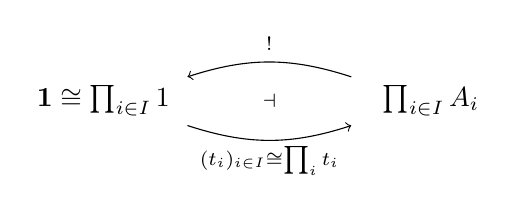
\begin{tikzpicture}[x=1.6em,y=1.6em]
  \node (L) at (0,0) {$\qcOne\cong\textstyle\prod_{i\in I}1$};
  \node (R) at (7.4,0) {$\textstyle\prod_{i\in I}A_{i}$};
  \draw[->] (5.6,0.55) to[bend right=18] (1.9,0.55);
  \node at (3.75,1.3) {$\scriptstyle !$};
  \node at (3.75,0.0) {$\scriptstyle\dashv$};
  \draw[->] (1.9,-0.55) to[bend right=18] (5.6,-0.55);
  \node at (3.75,-1.35) {$\scriptstyle(t_{i})_{i\in I}\cong\prod_{i}t_{i}$};
\end{tikzpicture}
\end{center}
它展示出 $(t_{i})_{i\in I}$ 是 $\prod_{i\in I}A_{i}$ 的一个终元素。由构造，
这个终元素被积锥的诸锥腿联合创生。特别地，诸积投影函子保持这个终元素，而且
由任何一族保持终元素的函子 $(f_{i}\colon X\to A_{i})_{i\in I}$ 诱导的、进入积
∞-范畴 $\prod_{i\in I}A_{i}$ 的映射也保持终元素。这就验证了子范畴
$\mathcal{K}_{\top}$ 对\trProduct{}封闭。

类似地，若 $A$ 是一个拥有终元素 $t\colon\qcOne\to A$ 的\trInfinityCategory{}，
则由命题 2.1.7(iii)，在 $t$ 处取常值的\trDiagram——我们仍把它记作 $t$——在
任何\trSimplicialSet{} $U$ 的\trCotensor{} $A^{U}$ 中定义一个终元素\footnote{原书
下方显示式右端印作 $\prod_{i\in I}A^{U}$，疑为上一显示式（积情形）之残留，
按上下文径改为 $A^{U}$。——译者注}
\begin{center}
\begin{tikzpicture}[x=1.6em,y=1.6em]
  \node (L) at (0,0) {$\qcOne\cong 1^{U}$};
  \node (R) at (6.0,0) {$A^{U}$};
  \draw[->] (4.4,0.55) to[bend right=18] (1.5,0.55);
  \node at (2.95,1.3) {$\scriptstyle !$};
  \node at (2.95,0.0) {$\scriptstyle\dashv$};
  \draw[->] (1.5,-0.55) to[bend right=18] (4.4,-0.55);
  \node at (2.95,-1.3) {$\scriptstyle t=t^{U}$};
\end{tikzpicture}
\end{center}
尚需论证：$A^{U}$ 中的终元素被极限锥的诸 0-箭头分量——亦即对余张量化单纯集
的每个顶点求值——联合创生。为此，设 $s\colon\qcOne\to A^{U}$ 具有如下性质：
对 $U$ 的每个顶点 $u$，
\[
s_{u}:=\quad
\qcOne\xrightarrow{\ \ s\ \ }A^{U}\xrightarrow{\ \mathrm{ev}_{u}\ }A
\]
在 $A$ 中是终的。由 $t\colon\qcOne\to A^{U}$ 的终端性，存在一个%
\trNaturalTransformation{} $\alpha\colon s\Rightarrow t$；由于 $s_{u}$ 与 $t$
都定义 $A$ 的终元素，$\alpha$ 在每个 $u$ 处的分量定义 $A$ 中的一个同构
$\alpha_{u}\colon s_{u}\cong t$。由推论 1.1.22，$\alpha$ 是一个同构，这告诉
我们 $s$ 也是 $A^{U}$ 的一个终元素。

归纳步骤考虑\trPullback{}图表
\begin{center}
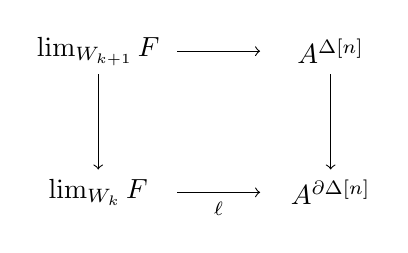
\begin{tikzpicture}[x=1.5em,y=1.5em]
  \node (TL) at (0,1.7) {$\lim_{W_{k+1}}F$};
  \node (TR) at (5.6,1.7) {$A^{\Delta[n]}$};
  \node (BL) at (0,-1.7) {$\lim_{W_{k}}F$};
  \node (BR) at (5.6,-1.7) {$A^{\partial\Delta[n]}$};
  \draw[->] (1.9,1.7) -- (3.9,1.7);
  \draw[->] (0,1.15) -- (0,-1.15);
  \node at (0.5,0.6) {$\scriptstyle\lrcorner$};
  \draw[->] (5.6,1.15) -- (5.6,-1.15);
  \draw[->] (1.9,-1.7) -- node[below]{$\scriptstyle\ell$} (3.9,-1.7);
\end{tikzpicture}
\end{center}
它由某个射影 $n$-胞腔的附接映射产生。归纳假设告诉我们 $\lim_{W_{k}}F$ 拥有
一个终元素 $t_{k}$，并且对 $i\in\partial\Delta[n]$ 的每个顶点，极限锥的相应
分量 $\ell_{i}\colon\lim_{W_{k}}F\to A$ 保持它。既然 $F$ 是一张取值于
$\mathcal{K}_{\top}$ 的图表，而 $A$ 是其像中的一个∞-范畴，我们知道 $A$ 必定
拥有一个终元素 $t\colon\qcOne\to A$。于是，常值图表
$t\colon\qcOne\to A^{\partial\Delta[n]}$ 在 $A^{\partial\Delta[n]}$ 中定义一个
终元素。由终端性，存在一个\trNaturalTransformation{}
$\alpha\colon\ell(t_{k})\Rightarrow t$，其在每个 $i\in\partial\Delta[n]$ 处的
分量都是 $A$ 中的同构。由推论 1.1.22，$\alpha$ 也是一个同构，这告诉我们
$\ell(t_{k})$ 也是 $A^{\partial\Delta[n]}$ 的一个终元素。如此便见 $\ell$ 保持
终元素。证明由下面这对引理完成。
\end{proof}

\begin{lemma}\label{lem:pullback-terminal-element}
考虑\trInfinityCategory{}的一个\trPullback{}图表
\begin{center}
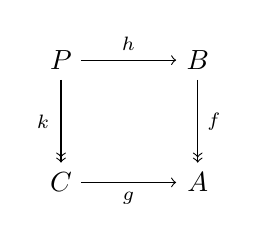
\begin{tikzpicture}[x=1.3em,y=1.3em]
  \node (P) at (0,1.7) {$P$};
  \node (B) at (3.8,1.7) {$B$};
  \node (C) at (0,-1.7) {$C$};
  \node (A) at (3.8,-1.7) {$A$};
  \draw[->] (0.55,1.7) -- node[above]{$\scriptstyle h$} (3.2,1.7);
  \draw[->>] (0,1.15) -- (0,-1.15);
  \node at (0.5,0.6) {$\scriptstyle\lrcorner$};
  \node at (-0.5,0) {$\scriptstyle k$};
  \draw[->>] (3.8,1.15) -- node[right]{$\scriptstyle f$} (3.8,-1.15);
  \draw[->] (0.55,-1.7) -- node[below]{$\scriptstyle g$} (3.2,-1.7);
\end{tikzpicture}
\end{center}
其中\trInfinityCategory{} $A$、$B$ 与 $C$ 拥有终元素，且函子 $f$ 与 $g$ 保持
它们。那么 $P$ 拥有一个终元素，它由\trPullback{}锥的诸条腿 $h$ 与 $k$ 创生。
\end{lemma}

\begin{proof}
若 $b\colon\qcOne\to B$ 与 $c\colon\qcOne\to C$ 是终的，则终元素的唯一性蕴含
$f(b)\cong g(c)\in A$。利用 $f$ 是\trIsofibration{}这一事实，这个同构沿 $f$
有一个提升 $b'\cong b$，后者于是定义 $B$ 的另一个终元素。二元组 $(c,b')$ 现在
诱导 $P$ 的一个元素 $t$，我们断言它是终的。

为看清这一点，我们应用命题 4.3.13；该命题证明：$t$ 是 $P$ 的终元素，当且仅当
定义域投影函子 $p_{0}\colon\mathrm{Hom}_{P}(P,t)\twoheadrightarrow P$ 是一个%
\trTrivialFibration{}。由 $t$ 的构造，我们知道：对于元素 $ht=b'$、$kt=c$ 与
$fht=gkt$，相应的定义域投影函子都是\trTrivialFibration{}；此外，由超立方体拉回
引理，下述立方体的顶面与底面
\begin{center}
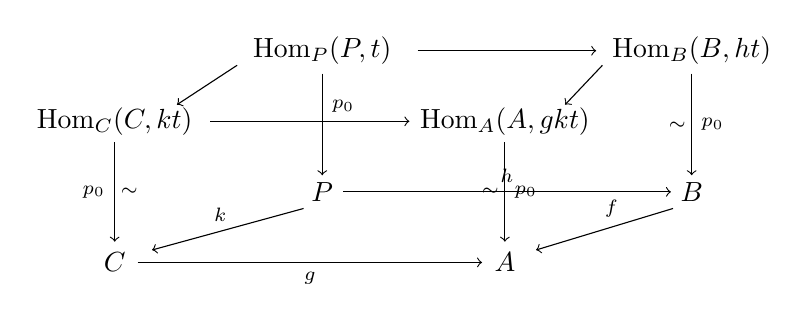
\begin{tikzpicture}[x=1.5em,y=1.5em]
  \node (HP) at (5.0,3.4) {$\mathrm{Hom}_{P}(P,t)$};
  \node (HB) at (13.9,3.4) {$\mathrm{Hom}_{B}(B,ht)$};
  \node (HC) at (0,1.7) {$\mathrm{Hom}_{C}(C,kt)$};
  \node (HA) at (9.4,1.7) {$\mathrm{Hom}_{A}(A,gkt)$};
  \draw[->] (7.3,3.4) -- (11.6,3.4);
  \draw[->] (2.3,1.7) -- (7.1,1.7);
  \draw[->] (2.95,3.05) -- (1.5,2.1);
  \draw[->] (11.75,3.05) -- (10.85,2.1);
  \draw[->] (5.0,2.85) -- node[right,pos=0.32]{$\scriptstyle p_{0}$} (5.0,0.4);
  \node at (5.5,2.4) {$\scriptstyle\lrcorner$};
  \draw[->] (13.9,2.85) -- node[right]{$\scriptstyle p_{0}$} (13.9,0.4);
  \node at (13.55,1.6) {$\scriptstyle\sim$};
  \draw[->] (0,1.2) -- node[left]{$\scriptstyle p_{0}$} (0,-1.2);
  \node at (0.35,0) {$\scriptstyle\sim$};
  \draw[->] (9.4,1.2) -- node[right]{$\scriptstyle p_{0}$} (9.4,-1.2);
  \node at (9.05,0) {$\scriptstyle\sim$};
  \node (P) at (5.0,0) {$P$};
  \node (B) at (13.9,0) {$B$};
  \node (C) at (0,-1.7) {$C$};
  \node (A) at (9.4,-1.7) {$A$};
  \draw[->] (5.5,0) -- node[above]{$\scriptstyle h$} (13.4,0);
  \draw[->] (4.55,-0.4) -- node[above,pos=0.55]{$\scriptstyle k$} (0.9,-1.4);
  \draw[->] (13.45,-0.4) -- node[above,pos=0.45]{$\scriptstyle f$} (10.15,-1.4);
  \draw[->] (0.55,-1.7) -- node[below]{$\scriptstyle g$} (8.85,-1.7);
  \node at (5.55,-0.45) {$\scriptstyle\lrcorner$};
\end{tikzpicture}
\end{center}
都是\trPullback。由命题 3.3.4，诸\trCospan{}之间的三支映射都是\trEquivalence{}这一事实
蕴含它们的\trPullback{}之间的映射也是\trEquivalence{}，正如所求。
\end{proof}

\begin{lemma}\label{lem:tower-terminal-element}
考虑\trIsofibration{}的一座塔
\[
A:=\lim\Big(\ \cdots\longrightarrow A_{n}
\xrightarrow{\ q_{n}\ }A_{n-1}
\longrightarrow\cdots
\longrightarrow A_{1}
\xrightarrow{\ q_{1}\ }A_{0}\ \Big)
\]
其中每个∞-范畴都拥有一个终元素，且塔中每支纤维化都保持终元素。那么塔的极限
拥有一个由极限锥的诸锥腿创生的终元素。
\end{lemma}

\begin{proof}
假设提供了终元素 $s_{n}\colon\qcOne\to A_{n}$ 使得 $q_{n}s_{n}\cong s_{n-1}$。
自塔的底端开始归纳地提升消去这些同构，便可选取另一族终元素
$t_{n}\colon\qcOne\to A_{n}$ 使得 $q_{n}t_{n}=t_{n-1}$。这个锥随即在极限 $A$
中诱导一个元素 $t\colon\qcOne\to A$，我们断言它是终的。这由命题 4.3.13 以及
下述观察得到：$p_{0}\colon\mathrm{Hom}_{A}(A,t)\twoheadrightarrow A$ 是等价
纤维化的∞-宇宙中一座塔的极限，此塔的对象是诸\trTrivialFibration{}
$p_{0}\colon\mathrm{Hom}_{A_{n}}(A_{n},t_{n})\twoheadrightarrow A_{n}$。由
\cref{prop:trivial-fibration-cosmoi}，
$p_{0}\colon\mathrm{Hom}_{A}(A,t)\twoheadrightarrow A$ 便也是一个%
\trTrivialFibration{}。
\end{proof}

把\cref{prop:terminal-element-cosmos}的结果应用于 $\mathcal{K}^{co}$ 便构造出
一个∞-宇宙 $\mathcal{K}_{\perp}$，其对象是 $\mathcal{K}$ 中拥有始对象的%
\trInfinityCategory{}，其 0-箭头是保持始元素的函子。不难验证：包含
$\mathcal{K}_{\perp}\hookrightarrow\mathcal{K}$ 是一个\trCosmologicalEmbedding{}。
\footnote{此处构造的诸∞-宇宙的其他对偶可类似地确立（见\cref{ex:lari-codual}）。}
合并这些结果，我们便为定义 4.4.1 的\trPointed{}\trInfinityCategory——即拥有%
\trZeroElement{}的那些∞-范畴——得到了一个∞-宇宙。

\begin{proposition}\label{prop:pointed-cosmos}
对任何\trInfinityCosmos{} $\mathcal{K}$，令 $\mathcal{K}_{*}$ 表示由%
\trPointed{}\trInfinityCategory——即拥有\trZeroElement{}的∞-范畴——与保持
它们的函子构成的拟范畴式富集范畴。那么包含 $\mathcal{K}_{*}\hookrightarrow\mathcal{K}$
是一个\trCosmologicalEmbedding{}，从 $\mathcal{K}$ 在 $\mathcal{K}_{*}$ 上创生
一个∞-宇宙结构，而且进一步：对 $\mathcal{K}_{*}$ 中定义为该∞-宇宙中某张图表之%
\trFlexibleWeightedLimit{}的每个对象，其\trZeroElement{}由极限锥的诸 0-箭头
锥腿创生。
\end{proposition}

\begin{proof}
此结果直接由\cref{prop:terminal-element-cosmos}及其对偶得到，因为由 $\mathcal{K}$
中拥有零对象的∞-范畴构成的∞-宇宙 $\mathcal{K}_{*}$ 同构于
$(\mathcal{K}_{\top})_{\perp}\cong(\mathcal{K}_{\perp})_{\top}$，其要义在于：
$\mathcal{K}_{\top}$ 中的始元素 $a\colon\qcOne\to A$ 由一个保持终元素的函子
编码，而这恰好说明 $a$ 是 $A$ 中的一个\trZeroElement{}。
\end{proof}

把\cref{prop:terminal-element-cosmos}的结果或其对偶应用于 $B\in\mathcal{K}$
之上\trIsofibration{}的∞-宇宙 $\mathcal{K}_{/B}$，我们得到两个令人感兴趣的新
∞-宇宙。

\begin{corollary}\label{cor:sliced-rari-lari}
对\trInfinityCosmos{} $\mathcal{K}$ 中任何\trInfinityCategory{} $B$，%
\trSliceInfinityCosmos{} $\mathcal{K}_{/B}$ 容有\trCosmologicalEmbedding{}的
∞-宇宙
\[
\Rari(\mathcal{K})_{/B}\hookrightarrow\mathcal{K}_{/B}
\hookleftarrow\Lari(\mathcal{K})_{/B}
\]
其对象分别是容有\trRightAdjoint{}右逆或\trLeftAdjoint{}右逆的 $B$ 之上的\trIsofibration{}；其 0-箭头
是 $B$ 之上的函子，它们与相应的\trRightAdjoint{}或\trLeftAdjoint{}交换，至相差 $B$ 之上的%
\trFiberedIsomorphism{}。
\end{corollary}

\begin{proof}
由引理 3.6.9，这两个∞-宇宙定义为
\[
\Rari(\mathcal{K})_{/B}:=(\mathcal{K}_{/B})_{\top}
\qquad\text{与}\qquad
\Lari(\mathcal{K})_{/B}:=(\mathcal{K}_{/B})_{\perp}.
\]
\end{proof}

利用\cref{cor:sliced-rari-lari}，我们可以确立类似的\trCosmologicalEmbedding
\[
\Rari(\mathcal{K})\hookrightarrow\mathcal{K}^{\dagger}
\hookleftarrow\Lari(\mathcal{K})
\]
它们定义由变底座的\trRightAdjoint{}右逆伴随或\trLeftAdjoint{}右逆伴随构成的∞-宇宙。为应用
\cref{prop:cosmologically-embedded}，我们必须检验对\trFlexibleWeightedLimit{}%
的封闭性。我们分别论证：对\trCotensor{}的论证容易，而对诸锥形极限的论证较难
——尝试过用定理 5.2.8(ii) 求解练习 5.2.iii 的读者或许已经发现了这一点。为
一次处理全部锥形极限，我们诉诸一条一般的 1-范畴论结果：它由底范畴
$\mathcal{B}$ 中的极限与各纤维 $\mathcal{E}_{B}$ 中的极限，构造出 Grothendieck
纤维化 $P\colon\mathcal{E}\to\mathcal{B}$ 的全空间 $\mathcal{E}$ 中的极限。

\begin{lemma}\label{lem:grothendieck-fibration-limits}
设 $P\colon\mathcal{E}\to\mathcal{B}$ 是 1-范畴之间的一个 Grothendieck 纤维化。
设 $\mathcal{J}$ 是一个小范畴，$D\colon\mathcal{J}\to\mathcal{E}$ 是一张图表，
并设：
\begin{itemize}
\item[(i)] 图表 $PD\colon\mathcal{J}\to\mathcal{B}$ 在 $\mathcal{B}$ 中拥有
一个\trLimit{} $L$ 及极限锥 $\lambda\colon\Delta L\Rightarrow PD$；
\item[(ii)] 把锥 $\lambda$ 提升为一个笛卡尔自然变换
$\chi\colon\lambda^{*}D\Rightarrow D$ 而构造出的图表
$\lambda^{*}D\colon\mathcal{J}\to\mathcal{E}_{L}$
\begin{center}
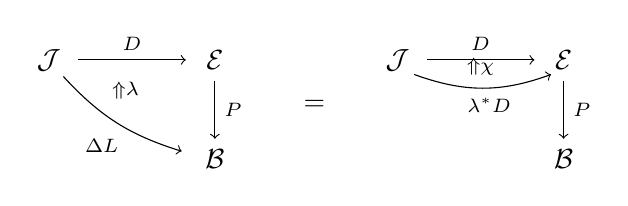
\begin{tikzpicture}[x=1.5em,y=1.5em]
  \begin{scope}[shift={(0,0)}]
  \node (J1) at (0,1.1) {$\mathcal{J}$};
  \node (E1) at (4.0,1.1) {$\mathcal{E}$};
  \node (B1) at (4.0,-1.3) {$\mathcal{B}$};
  \draw[->] (0.7,1.1) -- node[above]{$\scriptstyle D$} (3.3,1.1);
  \draw[->] (4.0,0.6) -- node[right]{$\scriptstyle P$} (4.0,-0.8);
  \draw[->] (0.35,0.7) to[bend right=15] node[below left,pos=0.6]{$\scriptstyle\Delta L$} (3.2,-1.1);
  \node at (1.85,0.35) {$\scriptstyle\Uparrow\lambda$};
  \end{scope}
  \node at (6.4,0) {$=$};
  \begin{scope}[shift={(8.4,0)}]
  \node (J2) at (0,1.1) {$\mathcal{J}$};
  \node (E2) at (4.0,1.1) {$\mathcal{E}$};
  \node (B2) at (4.0,-1.3) {$\mathcal{B}$};
  \draw[->] (0.7,1.1) -- node[above]{$\scriptstyle D$} (3.3,1.1);
  \draw[->] (4.0,0.6) -- node[right]{$\scriptstyle P$} (4.0,-0.8);
  \draw[->] (0.4,0.75) to[bend right=20] node[below,pos=0.55]{$\scriptstyle\lambda^{*}D$} (3.7,0.75);
  \node at (2.0,0.93) {$\scriptstyle\Uparrow\chi$};
  \end{scope}
\end{tikzpicture}
\end{center}
在纤维 $\mathcal{E}_{L}$ 中拥有一个\trLimit{} $M$ 及极限锥
$\mu\colon\Delta M\Rightarrow\lambda^{*}D$；
\item[(iii)] 极限锥 $\mu\colon\Delta M\Rightarrow\lambda^{*}D$ 被与 $\mathcal{B}$
中任何箭头 $u\colon B\to L$ 相关联的重标引函子 $u^{*}\colon\mathcal{E}_{L}\to\mathcal{E}_{B}$
所保持。
\end{itemize}
那么复合锥 $\Delta M\xRightarrow{\ \mu\ }\lambda^{*}D\xRightarrow{\ \chi\ }D$
展示出 $M$ 是 $\mathcal{E}$ 中图表 $D$ 的一个\trLimit{}。
\end{lemma}

\begin{proof}
Grothendieck 纤维化 $P\colon\mathcal{E}\to\mathcal{B}$ 定义域中的任何箭头
$f\colon E\to E'$ 都在同构的意义下唯一地分解为纤维 $\mathcal{E}_{PE}$ 中的
一支「竖直」箭头继以一支余定义域为 $E'$ 的 $Pf$ 之「水平」笛卡尔提升。

给定 $D$ 之上一个顶点为 $E\in\mathcal{E}$ 的锥
$\alpha\colon\Delta E\Rightarrow D$，由 (i)，其像
$P\alpha\colon\Delta PE\Rightarrow PD$ 经由一个映射 $b\colon PE\to L\in\mathcal{B}$
穿过极限锥 $\lambda\colon\Delta L\Rightarrow PD$\footnote{原书印作
「$\lambda\colon\Delta L\Rightarrow D$」，疑漏 $P$；按本引理 (i) 之极限锥
$\lambda\colon\Delta L\Rightarrow PD$ 径改。——译者注}唯一地分解。由 (ii) 中构造的
$\lambda$ 的笛卡尔提升 $\chi$ 的\trUniversalProperty{}，$\alpha$ 经由一个%
\trNaturalTransformation{} $\beta\colon\Delta E\Rightarrow\lambda^{*}D$ 穿过 $\chi$
唯一地分解，使得 $P\beta=\Delta b$。这个锥在同构的意义下唯一地分解为一个
「竖直」\trNaturalTransformation{} $\gamma\colon\Delta E\Rightarrow b^{*}\lambda^{*}D$
继以 $b$ 的一支「水平」笛卡尔提升。由 (iii)，$\mathcal{E}_{L}$ 中的极限锥
$\mu\colon\Delta M\Rightarrow\lambda^{*}D$ 沿 $b$ 拉回得到 $\mathcal{E}_{PE}$
中的一个极限锥，$\beta$ 的\trPullback{}经由一个映射 $k\colon E\to b^{*}M$ 穿过它分解。
于是，$\beta$ 本身经由这个映射 $k\colon E\to b^{*}M$ 与提升 $b\colon PE\to L$
的笛卡尔箭头 $b^{*}M\to M$ 之复合穿过 $\mu$ 唯一地分解。
\end{proof}

例如，余定义域投影函子 $\mathrm{cod}\colon\mathcal{K}^{\dagger}\to\mathcal{K}$
是底 1-范畴层面的一个 Grothendieck 纤维化，其 cod-笛卡尔提升由\trPullback{}方块定义。
既然\trIsofibration{}的\trRightAdjoint{}右逆可以构造为\trFiberedAdjunction（引理 3.6.9），而\trFiberedAdjunction{}%
在\trPullback{}下稳定（引理 3.6.6），这个 Grothendieck 纤维化便限制而定义一个
Grothendieck 纤维化 $\mathrm{cod}\colon\Rari(\mathcal{K})\to\mathcal{K}$，这使
得我们能够在下述结果的证明中求助于\cref{lem:grothendieck-fibration-limits}。

\begin{proposition}\label{prop:rari-lari-cosmoi}
对任何\trInfinityCosmos{} $\mathcal{K}$，\trIsofibration{}的∞-宇宙容有%
\trCosmologicalEmbedding{}的∞-宇宙
\[
\Rari(\mathcal{K})\hookrightarrow\mathcal{K}^{\dagger}
\hookleftarrow\Lari(\mathcal{K})
\]
其对象分别是容有\trRightAdjoint{}右逆或\trLeftAdjoint{}右逆的\trIsofibration{}；其 0-箭头分别是诸%
\trRightAdjoint{}之间的或诸\trLeftAdjoint{}之间的交换方块，其对应为同构。
\end{proposition}

我们把诸\trRightAdjoint{}之间其对应为同构的交换方块称为一个\textbf{\trExactSquare}（exact
square）。

\begin{proof}
由命题 B.3.8 与练习 B.4.i，拟范畴式富集子范畴 $\Rari(\mathcal{K})$ 在
$\mathcal{K}^{\dagger}$ 中是充盈的，于是由\cref{prop:cosmologically-embedded}
我们只需检验 $\Rari(\mathcal{K})\hookrightarrow\mathcal{K}^{\dagger}$ 对%
\trFlexibleWeightedLimit{}的封闭性。我们分别论证\trCotensor{}与诸锥形极限。

若 $p\colon E\twoheadrightarrow B$ 是 $\mathcal{K}$ 中一支容有\trRightAdjoint{}右逆的%
\trIsofibration{}，而 $U$ 是一个\trSimplicialSet{}，则\trCosmologicalFunctor{}
$(-)^{U}\colon\mathcal{K}\to\mathcal{K}$ 把这批数据送到
$p^{U}\colon E^{U}\twoheadrightarrow B^{U}$ 的一个\trRightAdjoint{}右逆，这就证明了
$\Rari(\mathcal{K})$ 中对象在 $\mathcal{K}^{\dagger}$ 中的单纯\trCotensor{}%
落在 $\Rari(\mathcal{K})$ 中。为断定 $\Rari(\mathcal{K})$ 在 $\mathcal{K}^{\dagger}$
中对单纯\trCotensor{}封闭，我们还须验证 $p^{U}$ 拥有 $\Rari(\mathcal{K})$ 中
单纯\trCotensor{}的富集\trUniversalProperty{}：也就是说，我们必须证明
$\mathcal{K}^{\dagger}$ 中\trFunctorSpace{}的自然同构
$\Fun(q,p^{U})\cong\Fun(q,p)^{U}$ 限制后定义 $\Rari(\mathcal{K})$ 中%
\trFunctorSpace{}的一个自然同构。由于包含 $\Rari(\mathcal{K})\hookrightarrow\mathcal{K}^{\dagger}$
在 0-箭头上为满，这等于验证 $\mathcal{K}^{\dagger}$ 中某些 0-箭头是%
\trExactSquare{}。

$\mathcal{K}^{\dagger}$ 中\trCotensor{} $p^{U}$ 的加权极限锥由单纯集的典范映射
$U\to\Fun(p^{U},p)$
给出，后者在每个顶点 $u\colon\qcOne\to U$ 上由
\begin{rveq}\label{eq:cotensor-cartesian-square}
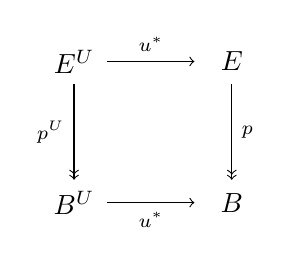
\begin{tikzpicture}[x=1.5em,y=1.5em]
  \node (TL) at (0,1.7) {$E^{U}$};
  \node (TR) at (3.8,1.7) {$E$};
  \node (BL) at (0,-1.7) {$B^{U}$};
  \node (BR) at (3.8,-1.7) {$B$};
  \draw[->] (0.8,1.7) -- node[above]{$\scriptstyle u^{*}$} (2.9,1.7);
  \draw[->>] (0,1.15) -- node[left]{$\scriptstyle p^{U}$} (0,-1.15);
  \draw[->>] (3.8,1.15) -- node[right]{$\scriptstyle p$} (3.8,-1.15);
  \draw[->] (0.8,-1.7) -- node[below]{$\scriptstyle u^{*}$} (2.9,-1.7);
\end{tikzpicture}
\end{rveq}
诸映射 $u^{*}$ 定义从 $(-)^{U}$ 到恒同函子的一个单纯自然变换的诸分量，于是这个
交换方块的对应是一个恒同，从而 $U$-\trCotensor{}的极限锥落在 $\Rari(\mathcal{K})$
中。最后，为验证 $\Rari(\mathcal{K})$ 中\trCotensor{}的\trUniversalProperty{}，
我们必须证明：任何交换方块——其定义域 $q$ 是一支容有\trRightAdjoint{}右逆的%
\trIsofibration
\begin{center}
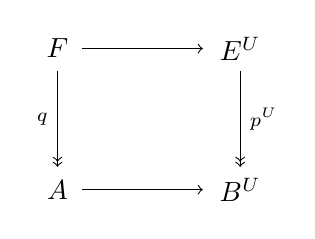
\begin{tikzpicture}[x=1.5em,y=1.5em]
  \node (TL) at (0,1.7) {$F$};
  \node (TR) at (4.4,1.7) {$E^{U}$};
  \node (BL) at (0,-1.7) {$A$};
  \node (BR) at (4.4,-1.7) {$B^{U}$};
  \draw[->] (0.6,1.7) -- (3.5,1.7);
  \draw[->>] (0,1.15) -- node[left]{$\scriptstyle q$} (0,-1.15);
  \draw[->>] (4.4,1.15) -- node[right]{$\scriptstyle p^{U}$} (4.4,-1.15);
  \draw[->] (0.6,-1.7) -- (3.5,-1.7);
\end{tikzpicture}
\end{center}
并且它与 \eqref{eq:cotensor-cartesian-square} 的每个方块复合均得\trExactSquare
——本身是正合的。为看清这一点，观察到恒同的对应定义一个\trNaturalTransformation{}，
后者由 $\Fun(A,E^{U})\cong\Fun(A,E)^{U}$ 中的一支 1-箭头表示，而假设说这支
1-箭头的诸分量对 $U$ 的每个顶点都是\trInvertible{}。推论 1.1.22 随即告诉我们
这支 1-箭头是\trInvertible{}，正如所求。

一个类似而稍容易的论证证明 $\Rari(\mathcal{K})$ 在 $\mathcal{K}^{\dagger}$ 中
对\trProduct{}封闭。只剩下证明这个子范畴对其余的锥形极限封闭。如上所论，
$\mathrm{cod}\colon\Rari(\mathcal{K})\to\mathcal{K}$ 是底 1-范畴层面的
Grothendieck 纤维化，其纤维是诸∞-宇宙 $\Rari(\mathcal{K})_{/B}$。由
\cref{lem:grothendieck-fibration-limits}，$\Rari(\mathcal{K})\subset\mathcal{K}^{\dagger}$
中的 1-范畴论极限锥可以计算为底中极限锥的笛卡尔提升与逐纤维图表的极限锥之
复合：在当前情形，做法是沿诸余定义域形成的极限锥拉回，然后在底图表的极限
对象之上的\trSliceInfinityCosmos{}中取\trLimit{}。由\cref{cor:sliced-rari-lari}，
这些 $\Rari(\mathcal{K})_{/B}$ 中图表在\trSliceInfinityCosmos{}
$\mathcal{K}_{/B}$ 中的逐纤维极限落在 $\Rari(\mathcal{K})_{/B}\hookrightarrow\Rari(\mathcal{K})$
中。此外，这些 1-范畴论极限被单纯\trCotensor{}保持，由命题 A.5.5，这意味着
它们的\trUniversalProperty{}富集化而定义锥形极限。由此我们见到
$\Rari(\mathcal{K})\hookrightarrow\mathcal{K}^{\dagger}$ 对%
\trFlexibleWeightedLimit{}封闭，从而如所断言定义一个\trCosmologicalEmbedding{}。
\end{proof}

既然我们已经确立了许多∞-宇宙与\trCosmologicallyEmbedded{}充盈子范畴的例子，便可以利用
下述结果：

\begin{proposition}\label{prop:pullback-cosmos}
设 $F\colon\mathcal{K}'\to\mathcal{K}$ 是一个\trCosmologicalFunctor{}，而
$\mathcal{L}\subset\mathcal{K}$ 是一个定义出\trCosmologicalEmbedding{}的
∞-宇宙的充盈子范畴。那么由\trPullback
\begin{center}
\begin{tikzpicture}[x=1.5em,y=1.5em]
  \node (TL) at (0,1.7) {$\mathcal{L}'$};
  \node (TR) at (3.4,1.7) {$\mathcal{L}$};
  \node (BL) at (0,-1.7) {$\mathcal{K}'$};
  \node (BR) at (3.4,-1.7) {$\mathcal{K}$};
  \draw[->] (0.8,1.7) -- (2.6,1.7);
  \draw[right hook->] (0,1.15) -- (0,-1.15);
  \node at (0.5,0.6) {$\scriptstyle\lrcorner$};
  \draw[right hook->] (3.4,1.15) -- (3.4,-1.15);
  \draw[->] (0.8,-1.7) -- node[above]{$\scriptstyle F$} (2.6,-1.7);
\end{tikzpicture}
\end{center}
定义的单纯富集范畴是充盈的，并定义 $\mathcal{K}'$ 的一个\trCosmologicalEmbedding{}的
子∞-宇宙，而且限制后的函子 $F\colon\mathcal{L}'\to\mathcal{L}$ 是宇宙论的。
\end{proposition}

\begin{proof}
\trPullback{} $\mathcal{L}'$ 的对象与 $n$-箭头定义为 $\mathcal{K}'$ 的那些在 $F$ 之下的
像落在单纯子范畴 $\mathcal{L}$ 中的对象与 $n$-箭头。特别地，由于包含
$\mathcal{L}\hookrightarrow\mathcal{K}$ 在正维箭头上为满，包含
$\mathcal{L}'\hookrightarrow\mathcal{K}'$ 亦然，从而特别地 $\mathcal{L}'$ 是拟
范畴式富集的。由于\trCosmologicalFunctor{} $F$ 保持诸\trEquivalence{}而
$\mathcal{L}\hookrightarrow\mathcal{K}$ 是充盈的，拟范畴式富集子范畴
$\mathcal{L}'$ 在 $\mathcal{K}'$ 中是充盈的，满足\cref{def:replete-subcategory}
的三个条件。

为证明充盈子范畴 $\mathcal{L}'\hookrightarrow\mathcal{K}'$ 容有一个由包含创生
的∞-宇宙结构，还须论证 $\mathcal{L}'$ 在 $\mathcal{K}'$ 中对%
\trFlexibleWeightedLimit{}封闭。考虑一张图表 $D\colon\mathcal{A}\to\mathcal{L}'$
与一个柔性权，并在 $\mathcal{L}$ 与 $\mathcal{K}'$ 中构造其%
\trFlexibleWeightedLimit{}。到 $\mathcal{K}$ 的函子把它们送到同一图表之上的一对
等价锥；由于包含 $\mathcal{L}\hookrightarrow\mathcal{K}$ 是充盈的，存在 $D$
之上的一个极限锥落在 $\mathcal{L}$ 中，其在 $\mathcal{K}$ 中的像等于
$\mathcal{K}'$ 中极限锥在函子 $F$ 之下的像。如今\trPullback{}的\trUniversalProperty{}%
让我们把这个锥提升到 $\mathcal{L}'$\footnote{原书印作「lift this cone to
$\mathcal{L}$」，按上下文——\trPullback{}之\trUniversalProperty{}给出
$\mathcal{L}'$ 中的对象——径改为 $\mathcal{L}'$。——译者注}
中，而一个类似的论证表明提升后的锥是原图表之上的一个\trFlexibleWeightedLimit{}%
锥。由构造注意：$\mathcal{L}'$ 中的\trFlexibleWeightedLimit{}被到 $\mathcal{K}'$
与到 $\mathcal{L}$ 的两个函子保持。

\cref{prop:cosmologically-embedded}适用于断定
$\mathcal{L}'\hookrightarrow\mathcal{K}'$ 是一个\trCosmologicalEmbedding{}。由于
$\mathcal{L}'$ 中的诸\trIsofibration{}在 $\mathcal{K}'$ 中创生并被 $F$ 保持，
而 $\mathcal{L}\hookrightarrow\mathcal{K}$ 是一个\trCosmologicalEmbedding{}，限制
后的函子 $F\colon\mathcal{L}'\to\mathcal{L}$ 保持诸\trIsofibration{}。既然
$F\colon\mathcal{L}'\to\mathcal{L}$ 保持\trFlexibleWeightedLimit{}，便见这个函子
是宇宙论的。
\end{proof}

这一结果让我们得以构造更多令人感兴趣的∞-宇宙。

\begin{proposition}\label{prop:J-shaped-cosmoi}
对任何\trInfinityCosmos{} $\mathcal{K}$ 与\trSimplicialSet{} $J$，存在%
\trCosmologicalEmbedding{}的∞-宇宙
\[
\mathcal{K}_{\top,J}\hookrightarrow\mathcal{K}\hookleftarrow\mathcal{K}_{\perp,J}
\]
\begin{itemize}
\item 其对象分别是 $\mathcal{K}$ 中容有全部形状为 $J$ 的\trLimit{}或全部形状
为 $J$ 的\trColimit{}的\trInfinityCategory{}；
\item 其 0-箭头是保持它们的诸函子。
\end{itemize}
而且进一步：对 $\mathcal{K}_{\top,J}$ 或 $\mathcal{K}_{\perp,J}$ 中定义为该
∞-宇宙中某张图表之\trFlexibleWeightedLimit{}的每个对象，其形状为 $J$ 的极限
或余极限分别由极限锥或余极限锥的诸 0-箭头锥腿创生。
\end{proposition}

\begin{proof}
就容有形状为 $J$ 的余极限的∞-范畴这一情形证明之，另一情形对偶。对任何取定的%
\trSimplicialSet{} $J$，存在一个\trCosmologicalFunctor{}
$F_{J}\colon\mathcal{K}\to\mathcal{K}^{\dagger}$：在对象上把一个∞-范畴 $A$ 送
到按 4.2.6 中的记号所得的\trIsofibration{}
$A^{J^{\triangleright}}\twoheadrightarrow A^{J}$，把一个函子 $f\colon A\to B$
送到交换方块
\begin{center}
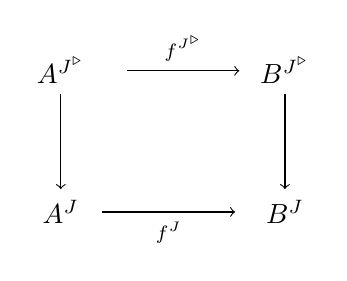
\begin{tikzpicture}[x=1.5em,y=1.5em]
  \node (TL) at (0,1.7) {$A^{J^{\triangleright}}$};
  \node (TR) at (5.4,1.7) {$B^{J^{\triangleright}}$};
  \node (BL) at (0,-1.7) {$A^{J}$};
  \node (BR) at (5.4,-1.7) {$B^{J}$};
  \draw[->] (1.6,1.7) -- node[above]{$\scriptstyle f^{J^{\triangleright}}$} (4.3,1.7);
  \draw[->] (0,1.15) -- (0,-1.15);
  \draw[->] (5.4,1.15) -- (5.4,-1.15);
  \draw[->] (1.0,-1.7) -- node[below]{$\scriptstyle f^{J}$} (4.2,-1.7);
\end{tikzpicture}
\end{center}
由推论 4.3.5，$A$ 容有形状为 $J$ 的余极限，当且仅当这支\trIsofibration{}容有
一个\trLeftAdjoint{}右逆；而 $f\colon A\to B$ 保持这些余极限，当且仅当上示方块是%
\trExactSquare{}。总而言之，拟范畴式富集子范畴 $\mathcal{K}_{\perp,J}$ 由\trPullback
\begin{center}
\begin{tikzpicture}[x=1.6em,y=1.5em]
  \node (TL) at (0,1.7) {$\mathcal{K}_{\perp,J}$};
  \node (TR) at (5.0,1.7) {$\Lari(\mathcal{K})$};
  \node (BL) at (0,-1.7) {$\mathcal{K}$};
  \node (BR) at (5.0,-1.7) {$\mathcal{K}^{\dagger}$};
  \draw[->] (1.5,1.7) -- (3.7,1.7);
  \draw[right hook->] (0,1.15) -- (0,-1.15);
  \node at (0.5,0.6) {$\scriptstyle\lrcorner$};
  \draw[right hook->] (5.0,1.15) -- (5.0,-1.15);
  \draw[->] (0.8,-1.7) -- node[above]{$\scriptstyle F_{J}$} (4.0,-1.7);
\end{tikzpicture}
\end{center}
定义。由\cref{prop:rari-lari-cosmoi}，
$\Lari(\mathcal{K})\hookrightarrow\mathcal{K}^{\dagger}$ 是一个%
\trCosmologicalEmbedding{}，于是\cref{prop:pullback-cosmos}证明包含
$\mathcal{K}_{\perp,J}\hookrightarrow\mathcal{K}$ 创生一个∞-宇宙结构，正如所
断言。

特别地，子范畴 $\mathcal{K}_{\perp,J}$ 在 $\mathcal{K}$ 中对%
\trFlexibleWeightedLimit{}的封闭性蕴含：定义为\trFlexibleWeightedLimit{}的
∞-范畴中形状为 $J$ 的余极限由极限锥的诸 0-箭头锥腿创生，如下所释。当然，
$\mathcal{K}_{\perp,J}$ 中一个∞-范畴的余极限——作为 $\mathcal{K}_{\perp,J}$
中诸∞-范畴的一张图表的加权极限而形成——被加权极限锥的诸 0-箭头锥腿保持，
因为 $\mathcal{K}_{\perp,J}$ 中的 0-箭头是保持形状为 $J$ 的余极限的函子。而且，
由于只要该图表落在子∞-宇宙 $\mathcal{K}_{\perp,J}$ 中，定义为 $\mathcal{K}$ 中%
\trFlexibleWeightedLimit{}的∞-范畴之 $J$-余极限完备性便可推出，这些 $J$-余
极限也是被创生的。
\end{proof}

\begin{proposition}\label{prop:cart-cocart-cosmoi}
对任何\trInfinityCosmos{} $\mathcal{K}$，\trIsofibration{}的∞-宇宙容有%
\trCosmologicalEmbedding{}的∞-宇宙
\[
\mathcal{C}\mathit{art}(\mathcal{K})\hookrightarrow\mathcal{K}^{\dagger}
\hookleftarrow\mathit{co}\mathcal{C}\mathit{art}(\mathcal{K})
\]
其对象分别是\trCartesianFibration{}或\trCocartesianFibration{}，其 0-箭头是\trCartesianFunctor。
类似地，对\trInfinityCosmos{} $\mathcal{K}$ 中任何\trInfinityCategory{} $B$，
\trSliceInfinityCosmos{} $\mathcal{K}_{/B}$ 容有\trCosmologicalEmbedding{}的
∞-宇宙
\[
\mathcal{C}\mathit{art}(\mathcal{K})_{/B}\hookrightarrow\mathcal{K}_{/B}
\hookleftarrow\mathit{co}\mathcal{C}\mathit{art}(\mathcal{K})_{/B}
\]
其对象分别是 $B$ 之上的\trCartesianFibration{}或\trCocartesianFibration{}，其 0-箭头是%
\trCartesianFunctor，诸∞-宇宙结构由诸包含创生。
\end{proposition}

\begin{proof}
由定理 5.2.8 与定理 5.3.4，拟范畴式富集范畴 $\mathcal{C}\mathit{art}(\mathcal{K})$
由\trPullback
\begin{center}
\begin{tikzpicture}[x=1.6em,y=1.5em]
  \node (TL) at (0,1.7) {$\mathcal{C}\mathit{art}(\mathcal{K})$};
  \node (TR) at (5.0,1.7) {$\Rari(\mathcal{K})$};
  \node (BL) at (0,-1.7) {$\mathcal{K}^{\dagger}$};
  \node (BR) at (5.0,-1.7) {$\mathcal{K}^{\dagger}$};
  \draw[->] (2.1,1.7) -- (3.6,1.7);
  \draw[right hook->] (0,1.15) -- (0,-1.15);
  \node at (0.5,0.6) {$\scriptstyle\lrcorner$};
  \draw[right hook->] (5.0,1.15) -- (5.0,-1.15);
  \draw[->] (1.0,-1.7) -- node[above]{$\scriptstyle K$} (4.0,-1.7);
\end{tikzpicture}
\end{center}
定义，\trPullback{}沿单纯函子 $K$ 进行，后者把一支\trIsofibration{}
$p\colon E\twoheadrightarrow B$ 送到\trIsofibration{}
$i_{1}\hat{\pitchfork}p\colon E^{\qcTwo}\twoheadrightarrow\mathrm{Hom}_{B}(B,p)$。
为看清这一点，回忆\cref{prop:rari-lari-cosmoi}：$\Rari(\mathcal{K})$ 的诸%
\trFunctorSpace{}中的 0-箭头是容有\trRightAdjoint{}右逆的诸\trIsofibration{}之间的交换
方块，使得恒同 2-胞腔的对应在涉及\trRightAdjoint{}的相应方块中诱导一个同构。由定理
5.3.4，这个条件沿函子 $K$ 拉回后告诉我们：$\mathcal{C}\mathit{art}(\mathcal{K})$
中的 0-箭头是诸\trCocartesianFibration{}之间的交换方块，它们按定义 5.3.2 的意义定义%
\trCartesianFunctor。

单纯函子 $K$ 由加权极限构造而来，因而保持一切加权极限。此外，它保持
\cref{prop:isofibration-cosmos}的诸\trIsofibration{}：若
$r\colon F\twoheadrightarrow P$ 是由始顶点到\cref{prop:isofibration-cosmos}(iii)
中所展示\trCospan{}之\trPullback{}的\trIsofibration{}，则它在函子 $K$ 的像之下对应的映射是
Leibniz 余张量 $i_{1}\hat{\pitchfork}r\colon F^{\qcTwo}\twoheadrightarrow\mathrm{Hom}_{P}(P,r)$。
于是，$K$ 是一个\trCosmologicalFunctor{}。由\cref{prop:pullback-cosmos}，包含
$\mathcal{C}\mathit{art}(\mathcal{K})\hookrightarrow\mathcal{K}^{\dagger}$ 创生
一个∞-宇宙结构。

我们有一张类似的\trPullback，它定义由固定底座的笛卡尔纤维化构成的拟范畴式富集范畴
\begin{center}
\begin{tikzpicture}[x=1.6em,y=1.5em]
  \node (CT) at (0,3.2) {$\mathcal{C}\mathit{art}(\mathcal{K})_{/B}$};
  \node (CU) at (6.4,3.2) {$\mathcal{C}\mathit{art}(\mathcal{K})$};
  \node (SL) at (0,1.0) {$\mathcal{K}_{/B}$};
  \node (DG) at (6.4,1.0) {$\mathcal{K}^{\dagger}$};
  \node (PT) at (0,-1.6) {$\qcOne$};
  \node (KK) at (6.4,-1.6) {$\mathcal{K}$};
  \draw[right hook->] (2.5,3.2) -- (4.3,3.2);
  \draw[right hook->] (0,2.6) -- (0,1.7);
  \node at (0.5,2.15) {$\scriptstyle\lrcorner$};
  \draw[right hook->] (6.4,2.6) -- (6.4,1.7);
  \draw[right hook->] (1.4,1.0) -- (5.3,1.0);
  \draw[->] (0,0.35) -- (0,-1.0);
  \node at (0.5,0.3) {$\scriptstyle\lrcorner$};
  \draw[->] (6.4,0.35) -- node[right]{$\scriptstyle\mathrm{cod}$} (6.4,-1.0);
  \draw[->] (0.7,-1.6) -- node[above]{$\scriptstyle B$} (5.6,-1.6);
\end{tikzpicture}
\end{center}
但我们不能求助于\cref{prop:pullback-cosmos}，因为包含
$\mathcal{K}_{/B}\hookrightarrow\mathcal{K}^{\dagger}$ 既非宇宙论亦不充盈。取
而代之，我们必须求助于\cref{prop:cosmologically-embedded}。由推论 5.3.1 与
定理 5.3.4，$\mathcal{C}\mathit{art}(\mathcal{K})_{/B}\hookrightarrow\mathcal{K}_{/B}$
是一个充盈子范畴。$\mathcal{C}\mathit{art}(\mathcal{K})_{/B}$ 与 $\mathcal{K}_{/B}$
中的连通锥形极限由到 $\mathcal{C}\mathit{art}(\mathcal{K})$ 与到
$\mathcal{K}^{\dagger}$ 的包含创生，所以它们由包含
$\mathcal{C}\mathit{art}(\mathcal{K})_{/B}\hookrightarrow\mathcal{K}_{/B}$ 创生。
只剩下直接论证：\trProduct{}与单纯\trCotensor{}被这个包含创生。

由命题 1.2.22，诸\trIsofibration{} $p_{i}\colon E_{i}\twoheadrightarrow B$ 之
积由\trPullback
\begin{center}
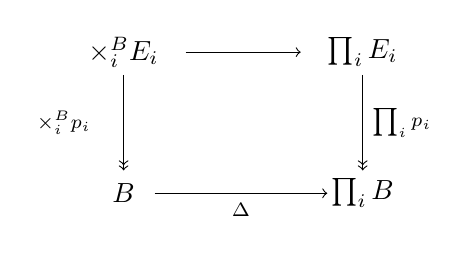
\begin{tikzpicture}[x=1.6em,y=1.5em]
  \node (TL) at (0,1.7) {$\times_{i}^{B}E_{i}$};
  \node (TR) at (5.4,1.7) {$\prod_{i}E_{i}$};
  \node (BL) at (0,-1.7) {$B$};
  \node (BR) at (5.4,-1.7) {$\prod_{i}B$};
  \draw[->] (1.4,1.7) -- (4.0,1.7);
  \draw[->>] (0,1.15) -- (0,-1.15);
  \node at (0.5,0.6) {$\scriptstyle\lrcorner$};
  \node at (-1.35,0) {$\scriptstyle\times_{i}^{B}p_{i}$};
  \draw[->>] (5.4,1.15) -- node[right]{$\scriptstyle\prod_{i}p_{i}$} (5.4,-1.15);
  \draw[->] (0.7,-1.7) -- node[below]{$\scriptstyle\Delta$} (4.6,-1.7);
\end{tikzpicture}
\end{center}
形成。若每支 $p_{i}$ 都是\trCartesianFibration{}，则由于
$\mathcal{C}\mathit{art}(\mathcal{K})$ 是一个∞-宇宙，$\prod_{i}p_{i}$ 仍是%
\trCartesianFibration，
且极限锥的诸锥腿是\trCartesianFunctor。由命题 5.2.4 可知：它们在 $\mathcal{K}_{/B}$ 中
的积是一个\trCartesianFibration{}，而且通过把\trPullback{}方块与诸积投影复合而定义的
极限锥诸锥腿是\trCartesianFunctor。由于笛卡尔变换由\trPullback{}创生，易得：以
$\times_{i}^{B}p_{i}$ 为余定义域的方块是\trCartesianFunctor，当且仅当以 $p_{i}$ 为余
定义域的每个复合方块都是\trCartesianFunctor。这就证明\trProduct{}由包含
$\mathcal{C}\mathit{art}(\mathcal{K})_{/B}\hookrightarrow\mathcal{K}_{/B}$ 创生。

类似地，由命题 1.2.22，一支\trIsofibration{} $p\colon E\twoheadrightarrow B$
与单纯集 $U$ 的\trCotensor{}由\trPullback
\begin{center}
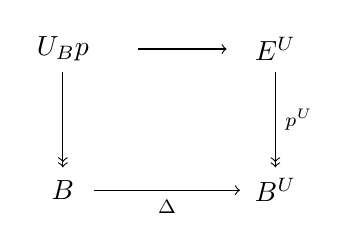
\begin{tikzpicture}[x=1.6em,y=1.5em]
  \node (TL) at (0,1.7) {$U\pitchfork_{B}p$};
  \node (TR) at (4.8,1.7) {$E^{U}$};
  \node (BL) at (0,-1.7) {$B$};
  \node (BR) at (4.8,-1.7) {$B^{U}$};
  \draw[->] (1.7,1.7) -- (3.7,1.7);
  \draw[->>] (0,1.15) -- (0,-1.15);
  \node at (0.5,0.6) {$\scriptstyle\lrcorner$};
  \draw[->>] (4.8,1.15) -- node[right]{$\scriptstyle p^{U}$} (4.8,-1.15);
  \draw[->] (0.7,-1.7) -- node[below]{$\scriptstyle\Delta$} (4.0,-1.7);
\end{tikzpicture}
\end{center}
形成，因而当 $p$ 是\trCartesianFibration{}时它也是。一个类似的论证表明这个
对象拥有 $\mathcal{C}\mathit{art}(\mathcal{K})_{/B}$ 中单纯\trCotensor{}所要求
的\trUniversalProperty{}，证明至此完成。
\end{proof}

诸笛卡尔纤维化的∞-宇宙为探索 Shah 所发展的参数化∞-范畴论 [115] 提供了一片
沃土。

\begin{proposition}\label{prop:discrete-cart-cosmoi}
对任何\trInfinityCosmos{} $\mathcal{K}$，存在\trCosmologicalEmbedding{}的
∞-宇宙
\begin{center}
\begin{tikzpicture}[x=1.25em,y=1.4em]
  \node (DC) at (0,1.6) {$\mathcal{D}isc\mathcal{C}\mathit{art}(\mathcal{K})$};
  \node (KG) at (8.6,1.6) {$\mathcal{K}^{\dagger}$};
  \node (DCC) at (17.2,1.6) {$\mathcal{D}iscco\mathcal{C}\mathit{art}(\mathcal{K})$};
  \node (C) at (4.3,-1.5) {$\mathcal{C}\mathit{art}(\mathcal{K})$};
  \node (CC) at (12.9,-1.5) {$\mathit{co}\mathcal{C}\mathit{art}(\mathcal{K})$};
  \draw[right hook->] (2.8,1.6) -- (6.2,1.6);
  \draw[right hook->] (14.4,1.6) -- (11.0,1.6);
  \draw[right hook->] (1.1,1.1) -- (3.3,-1.0);
  \draw[right hook->] (5.3,-1.0) -- (7.5,1.1);
  \draw[right hook->] (11.9,-1.0) -- (9.7,1.1);
  \draw[right hook->] (16.1,1.1) -- (13.9,-1.0);
\end{tikzpicture}
\end{center}
其对象是\trDiscreteCartesianFibration{}或\trDiscreteCocartesianFibration{}。类似地，对\trInfinityCosmos{}
$\mathcal{K}$ 中任何\trInfinityCategory{} $B$，存在\trCosmologicalEmbedding{}%
的∞-宇宙
\begin{center}
\begin{tikzpicture}[x=1.15em,y=1.4em]
  \node (DC) at (0,1.6) {$\mathcal{D}isc\mathcal{C}\mathit{art}(\mathcal{K})_{/B}$};
  \node (KG) at (9.6,1.6) {$\mathcal{K}_{/B}$};
  \node (DCC) at (19.2,1.6) {$\mathcal{D}iscco\mathcal{C}\mathit{art}(\mathcal{K})_{/B}$};
  \node (C) at (4.8,-1.5) {$\mathcal{C}\mathit{art}(\mathcal{K})_{/B}$};
  \node (CC) at (14.4,-1.5) {$\mathit{co}\mathcal{C}\mathit{art}(\mathcal{K})_{/B}$};
  \draw[right hook->] (3.4,1.6) -- (6.8,1.6);
  \draw[right hook->] (15.8,1.6) -- (12.4,1.6);
  \draw[right hook->] (1.3,1.1) -- (3.8,-1.0);
  \draw[right hook->] (5.8,-1.0) -- (8.5,1.1);
  \draw[right hook->] (13.4,-1.0) -- (10.7,1.1);
  \draw[right hook->] (18.1,1.1) -- (15.4,-1.0);
\end{tikzpicture}
\end{center}
其对象分别是 $B$ 之上的\trDiscreteCartesianFibration{}或\trDiscreteCocartesianFibration{}。
\end{proposition}

\begin{proof}
由\cref{ex:discrete-cart}，固定底座的离散纤维化之∞-宇宙作为离散对象的∞-宇宙
产生：
\[
\mathcal{D}isc\mathcal{C}\mathit{art}(\mathcal{K})_{/B}\cong
(\mathcal{C}\mathit{art}(\mathcal{K})_{/B})^{\approx}
\qquad\text{与}\qquad
\mathcal{D}iscco\mathcal{C}\mathit{art}(\mathcal{K})_{/B}\cong
(\mathit{co}\mathcal{C}\mathit{art}(\mathcal{K})_{/B})^{\approx}
\]
从而其存在性由\cref{prop:discrete-cosmos}保证。变底座的离散纤维化之∞-宇宙
作为\trPullback{}产生：
\begin{center}
\begin{tikzpicture}[x=1.6em,y=1.5em]
  \node (DC) at (0,1.6) {$\mathcal{D}isc\mathcal{C}\mathit{art}(\mathcal{K})$};
  \node (KG) at (8.6,1.6) {$\mathcal{K}^{\dagger}$};
  \node (DCC) at (17.2,1.6) {$\mathcal{D}iscco\mathcal{C}\mathit{art}(\mathcal{K})$};
  \node (C) at (0,-1.6) {$\mathcal{C}\mathit{art}(\mathcal{K})$};
  \node (KGb) at (8.6,-1.6) {$\mathcal{K}^{\dagger}$};
  \node (CC) at (17.2,-1.6) {$\mathit{co}\mathcal{C}\mathit{art}(\mathcal{K})$};
  \draw[->] (2.8,1.6) -- (5.9,1.6);
  \draw[->] (11.3,1.6) -- (14.4,1.6);
  \draw[right hook->] (0,1.0) -- (0,-0.9);
  \node at (0.5,0.35) {$\scriptstyle\lrcorner$};
  \draw[right hook->] (8.6,1.0) -- (8.6,-0.9);
  \draw[right hook->] (17.2,1.0) -- (17.2,-0.9);
  \node at (16.6,0.35) {$\scriptstyle\lrcorner$};
  \draw[->] (2.2,-1.6) -- node[above]{$\scriptstyle K$} (7.6,-1.6);
  \draw[->] (14.9,-1.6) -- node[above]{$\scriptstyle K$} (9.5,-1.6);
\end{tikzpicture}
\end{center}
沿\cref{prop:cart-cocart-cosmoi}之证明中定义的\trCosmologicalFunctor{} $K$ 的
限制进行\trPullback，从而由\cref{prop:pullback-cosmos}它们存在。
\end{proof}

\begin{proposition}\label{prop:stable-cosmos}
对任何\trInfinityCosmos{} $\mathcal{K}$，$\mathcal{K}$ 中由\trStable{}
\trInfinityCategory{}与\trExactFunctor{}构成的充盈子范畴 $\mathcal{S}tab(\mathcal{K})$
是一个∞-宇宙，且包含 $\mathcal{S}tab(\mathcal{K})\hookrightarrow\mathcal{K}$
是一个\trCosmologicalEmbedding{}。
\end{proposition}

回忆练习 4.4.iv：在此语境中，稳定∞-范畴之间的一个函子称为\textbf{正合}（exact）
的，恰当它保持\trZeroElement{}以及所谓的同时定义\trPushout{}与\trPullback{}%
的\trExactSquare{}。\footnote{译注：此「正合方块」与命题 6.3.10 所定义者
（伴随对应为同构之交换方块）同名异义，此处照录原书用词。}
\begin{proof}
简化\cref{prop:J-shaped-cosmoi}的记号，以 $\mathcal{K}_{\sqcup}$ 与
$\mathcal{K}_{\sqcap}$ 分别表示由 $\mathcal{K}$ 中容有\trPullback{}与\trPushout{}的∞-范畴构成
的∞-宇宙。我们论证：$(\mathcal{K}_{\sqcup})_{\sqcap}\cong(\mathcal{K}_{\sqcap})_{\sqcup}$
这两个∞-宇宙作为 $\mathcal{K}$ 的充盈子范畴是同构的。
$(\mathcal{K}_{\sqcup})_{\sqcap}$ 的一个对象是 $\mathcal{K}_{\sqcup}$ 中一个
容有伴随
\begin{center}
\begin{tikzpicture}[x=1.6em,y=1.6em]
  \node (L) at (0,0) {$A^{\square}$};
  \node (R) at (4.6,0) {$A^{\sqcap}$};
  \draw[->] (3.4,0.5) to[bend left=15] (1.2,0.5);
  \node at (2.3,1.15) {$\scriptstyle\mathrm{lan}$};
  \node at (2.3,0.0) {$\scriptstyle\dashv$};
  \draw[->] (1.2,-0.5) to[bend right=15] (3.4,-0.5);
  \node at (2.3,-1.15) {$\scriptstyle\mathrm{res}$};
\end{tikzpicture}
\end{center}
的∞-范畴 $A$，此伴随居于∞-宇宙 $\mathcal{K}_{\sqcup}$ 中，意思是函子
$\mathrm{lan}\colon A^{\sqcap}\to A^{\square}$ 保持这两个∞-范畴都容有的诸\trPullback。
既然 $A$ 本身容有\trPullback，$A^{\sqcap}$ 与 $A^{\square}$ 中的\trPullback{}便可以逐点定义，
经由伴随
\begin{center}
\begin{tikzpicture}[x=1.5em,y=1.6em]
  \node (L1) at (0,0) {$(A^{\sqcap})^{\square}$};
  \node (R1) at (5.2,0) {$(A^{\sqcap})^{\sqcup}$};
  \draw[->] (3.5,0.45) to[bend left=15] (1.7,0.45);
  \node at (2.6,1.0) {$\scriptstyle\mathrm{res}$};
  \node at (2.6,-0.05) {$\scriptstyle\dashv$};
  \draw[->] (1.7,-0.45) to[bend right=15] (3.5,-0.45);
  \node at (2.6,-1.05) {$\scriptstyle\mathrm{ran}^{\sqcap}$};
  \node at (8.0,0) {与};
  \node (L2) at (10.8,0) {$(A^{\square})^{\square}$};
  \node (R2) at (16.0,0) {$(A^{\square})^{\sqcup}$};
  \draw[->] (14.3,0.45) to[bend left=15] (12.5,0.45);
  \node at (13.4,1.0) {$\scriptstyle\mathrm{res}$};
  \node at (13.4,-0.05) {$\scriptstyle\dashv$};
  \draw[->] (12.5,-0.45) to[bend right=15] (14.3,-0.45);
  \node at (13.4,-1.05) {$\scriptstyle\mathrm{ran}^{\square}$};
\end{tikzpicture}
\end{center}
于是它们自动被限制函子保持。于是，「这个伴随居于 $\mathcal{K}_{\sqcup}$ 中」
这一条件等价于「典范\trNaturalTransformation
\begin{center}
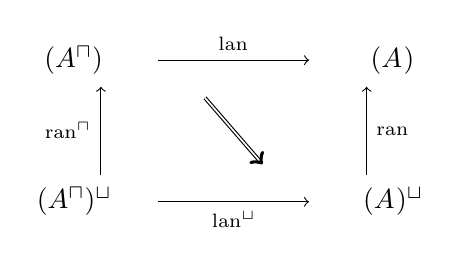
\begin{tikzpicture}[x=1.6em,y=1.6em]
  \node (TL) at (0,1.6) {$(A^{\sqcap})^{\square}$};
  \node (TR) at (7.2,1.6) {$(A^{\square})^{\square}$};
  \node (BL) at (0,-1.6) {$(A^{\sqcap})^{\sqcup}$};
  \node (BR) at (7.2,-1.6) {$(A^{\square})^{\sqcup}$};
  \draw[->] (1.9,1.6) -- node[above]{$\scriptstyle\mathrm{lan}^{\square}$} (5.3,1.6);
  \draw[->] (0.6,-1.0) -- node[left]{$\scriptstyle\mathrm{ran}^{\sqcap}$} (0.6,1.0);
  \draw[->] (6.6,-1.0) -- node[right]{$\scriptstyle\mathrm{ran}^{\square}$} (6.6,1.0);
  \draw[->] (1.9,-1.6) -- node[below]{$\scriptstyle\mathrm{lan}^{\sqcup}$} (5.3,-1.6);
  \draw[double,->] (2.95,0.75) -- (4.25,-0.75);
\end{tikzpicture}
\end{center}
是一个同构」这一条件。

对偶地，$(\mathcal{K}_{\sqcap})_{\sqcup}$ 的一个对象是容有\trPushout{}并且也容有伴随
\begin{center}
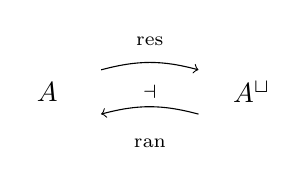
\begin{tikzpicture}[x=1.6em,y=1.6em]
  \node (L) at (0,0) {$A^{\square}$};
  \node (R) at (4.6,0) {$A^{\sqcup}$};
  \draw[->] (1.2,0.5) to[bend left=15] (3.4,0.5);
  \node at (2.3,1.15) {$\scriptstyle\mathrm{res}$};
  \node at (2.3,0.0) {$\scriptstyle\dashv$};
  \draw[->] (3.4,-0.5) to[bend right=15] (1.2,-0.5);
  \node at (2.3,-1.15) {$\scriptstyle\mathrm{ran}$};
\end{tikzpicture}
\end{center}
的∞-范畴 $A$，此伴随居于∞-宇宙 $\mathcal{K}_{\sqcap}$ 中，意思是\trPullback{}函子
$\mathrm{ran}\colon A^{\sqcup}\to A^{\square}$ 保持逐点定义的\trPushout，亦即：典范%
\trNaturalTransformation
\begin{center}
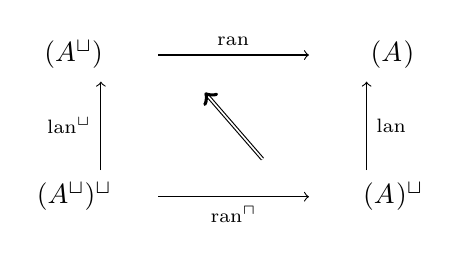
\begin{tikzpicture}[x=1.6em,y=1.6em]
  \node (TL) at (0,1.6) {$(A^{\sqcup})^{\square}$};
  \node (TR) at (7.2,1.6) {$(A^{\square})^{\square}$};
  \node (BL) at (0,-1.6) {$(A^{\sqcup})^{\sqcup}$};
  \node (BR) at (7.2,-1.6) {$(A^{\square})^{\sqcup}$};
  \draw[->] (1.9,1.6) -- node[above]{$\scriptstyle\mathrm{ran}^{\square}$} (5.3,1.6);
  \draw[->] (0.6,-1.0) -- node[left]{$\scriptstyle\mathrm{lan}^{\sqcup}$} (0.6,1.0);
  \draw[->] (6.6,-1.0) -- node[right]{$\scriptstyle\mathrm{lan}^{\square}$} (6.6,1.0);
  \draw[->] (1.9,-1.6) -- node[below]{$\scriptstyle\mathrm{ran}^{\sqcap}$} (5.3,-1.6);
  \draw[double,->] (4.25,-0.75) -- (2.95,0.75);
\end{tikzpicture}
\end{center}
是一个同构。于是我们见到 $(\mathcal{K}_{\sqcup})_{\sqcap}$ 与
$(\mathcal{K}_{\sqcap})_{\sqcup}$ 的对象相重合。类似地，$(\mathcal{K}_{\sqcup})_{\sqcap}$
与 $(\mathcal{K}_{\sqcap})_{\sqcup}$ 中的 0-箭头都是既保持\trPullback{}又保持\trPushout{}的
函子。这就证明 $(\mathcal{K}_{\sqcup})_{\sqcap}$ 与 $(\mathcal{K}_{\sqcap})_{\sqcup}$
如所断言定义 $\mathcal{K}$ 的同构子范畴。一个类似而更简单的观察为
\cref{prop:pointed-cosmos}之证明中断言的
$(\mathcal{K}_{\top})_{\perp}\cong(\mathcal{K}_{\perp})_{\top}$ 提供了理由。

由定理 4.4.12(iii)，一个∞-范畴是稳定的，恰当它带点、容有\trPullback{}与\trPushout、\trPullback{}函子
保持\trPushout、且\trPushout{}函子保持\trPullback。由定理 4.4.12(iii)$\Rightarrow$(ii) 之证明，
这些条件蕴含\trPullback{}方块与\trPushout{}方块相重合。由此我们见到 $\mathcal{S}tab(\mathcal{K})$
是
\begin{center}
\begin{tikzpicture}[x=1.5em,y=1.5em]
  \node (TL) at (0,1.7) {$\mathcal{S}tab(\mathcal{K})$};
  \node (TR) at (8.2,1.7)
    {$(\mathcal{K}_{\sqcup})_{\sqcap}\cong(\mathcal{K}_{\sqcap})_{\sqcup}$};
  \node (BL) at (0,-1.7)
    {$(\mathcal{K}_{\top})_{\perp}\cong(\mathcal{K}_{\perp})_{\top}$};
  \node (BR) at (8.2,-1.7) {$\mathcal{K}$};
  \draw[right hook->] (2.2,1.7) -- (3.6,1.7);
  \draw[right hook->] (0,1.15) -- (0,-1.15);
  \node at (0.5,0.6) {$\scriptstyle\lrcorner$};
  \draw[right hook->] (8.2,1.15) -- (8.2,-1.15);
  \draw[->] (3.4,-1.7) -- (6.0,-1.7);
\end{tikzpicture}
\end{center}
这个\trCosmologicalEmbedding{}的∞-宇宙之交，从而由\cref{prop:pullback-cosmos}
它本身是一个\trCosmologicalEmbedding{}的∞-宇宙。
\end{proof}

本节的结果可用于证明∞-范畴论文献中的技术性结果（见\cref{ex:cocartesian-pullback}）。
我们以沿这条路线的若干结果为例作结。

\begin{lemma}\label{lem:pullback-limit-creation}
考虑\trInfinityCategory{}的一个\trPullback{}图表，其竖直函子为\trIsofibration{}：
\begin{center}
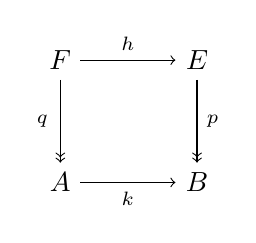
\begin{tikzpicture}[x=1.3em,y=1.3em]
  \node (F) at (0,1.7) {$F$};
  \node (E) at (3.8,1.7) {$E$};
  \node (A) at (0,-1.7) {$A$};
  \node (B) at (3.8,-1.7) {$B$};
  \draw[->] (0.55,1.7) -- node[above]{$\scriptstyle h$} (3.2,1.7);
  \draw[->>] (0,1.15) -- (0,-1.15);
  \node at (0.5,0.6) {$\scriptstyle\lrcorner$};
  \node at (-0.5,0) {$\scriptstyle q$};
  \draw[->>] (3.8,1.15) -- node[right]{$\scriptstyle p$} (3.8,-1.15);
  \draw[->] (0.55,-1.7) -- node[below]{$\scriptstyle k$} (3.2,-1.7);
\end{tikzpicture}
\end{center}
那么凡 $k$ 保持且 $p$ 创生的任一类\trLimit{}或\trColimit{}，$q$ 皆创生而 $h$ 皆
保持。
\end{lemma}

\begin{proof}
这些假设保证\trPullback{}的底\trCospan{}落在\cref{prop:J-shaped-cosmoi}的∞-宇宙中。既然这
是一个\trCosmologicalEmbedding{}的∞-宇宙，∞-范畴的\trPullback{}也落在其中，这告诉我
们：凡在 $E$、$A$ 与 $B$ 中存在且被 $p$ 与 $k$ 保持的极限或余极限，$F$ 都容有，
且 $q$ 与 $h$ 都保持。

只剩下论证这些（余）极限由 $q\colon F\twoheadrightarrow A$ 创生。设
$d\colon\mathcal{D}\to F^{J}$ 是一族图表，而 $\eta\colon d\Rightarrow\Delta c$
是此图表之下的一个锥，使得 $q\eta$ 是 $qd$ 在 $A$ 中的一个余极限锥。那么
$kq\eta=ph\eta$ 是 $kqd=phd$ 在 $B$ 中的一个余极限锥。既然假定
$p\colon E\twoheadrightarrow B$ 创生余极限，这便告诉我们 $h\eta$ 是 $hd$ 在
$E$ 中的一个余极限锥。如今\cref{prop:J-shaped-cosmoi}的第二条论断——它告诉我
们 $F$ 中的（余）极限由函子 $q$ 与 $h$ 联合创生——让我们得以断定 $\eta$ 是
$F$ 中的一个余极限锥，正如所断言。
\end{proof}

我们的最后一个应用重证一条与\trStable{}\trInfinityCategory{}之理论相关的结果
[80, 1.4.2.24]。

\begin{lemma}\label{lem:spa-stable}
设 $A$ 是一个容有\trPullback{}的\trPointed{}\trInfinityCategory{}。那么\trLoops{}函子之塔的
同伦极限定义一个\trStable{}\trInfinityCategory{}。
\[
\mathrm{Sp}A:=\lim\Big(\ \cdots\longrightarrow A
\xrightarrow{\ \Omega\ }A
\xrightarrow{\ \Omega\ }A
\xrightarrow{\ \Omega\ }A\ \Big)
\]
\end{lemma}

\begin{proof}
由于诸\trLoops{}函子不是\trIsofibration{}，\trLoops{}函子之塔的同伦极限这样计算：先把每支
映射换成所在的∞-宇宙 $\mathcal{K}$ 中的一支\trIsofibration{}，然后取逆向极限。
或者，由\cref{lem:iso-towers-flexible}与\ref{lem:iso-towers-inverse-limits}，
$\mathrm{Sp}A$ 由同构塔
\begin{rveq}\label{eq:spa-iso-tower}
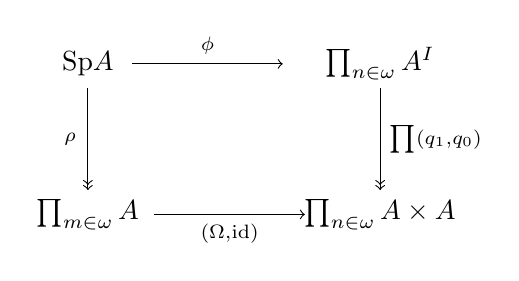
\begin{tikzpicture}[x=1.6em,y=1.6em]
  \node (TL) at (0,1.7) {$\mathrm{Sp}A$};
  \node (TR) at (6.6,1.7) {$\prod_{n\in\omega}A^{\hciso}$};
  \node (BL) at (0,-1.7) {$\prod_{m\in\omega}A$};
  \node (BR) at (6.6,-1.7) {$\prod_{n\in\omega}A\times A$};
  \draw[->] (1.0,1.7) -- node[above]{$\scriptstyle\phi$} (4.4,1.7);
  \draw[->>] (0,1.15) -- (0,-1.15);
  \node at (0.5,0.6) {$\scriptstyle\lrcorner$};
  \node at (-0.4,0) {$\scriptstyle\rho$};
  \draw[->>] (6.6,1.15) -- node[right]{$\scriptstyle\prod(q_{1},q_{0})$} (6.6,-1.15);
  \draw[->] (1.5,-1.7) -- node[below]{$\scriptstyle(\Omega,\mathrm{id})$} (4.9,-1.7);
\end{tikzpicture}
\end{rveq}
定义，它把 $\mathrm{Sp}A$ 定义为装备有一个锥
\begin{center}
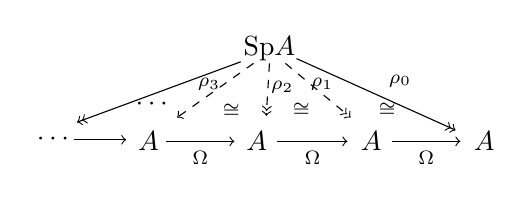
\begin{tikzpicture}[x=1.15em,y=1.15em]
  \node (SpA) at (7.1,3.6) {$\mathrm{Sp}A$};
  \node (dots0) at (0.3,0.75) {$\cdots$};
  \node (A1) at (3.3,0.7) {$A$};
  \node (A2) at (6.7,0.7) {$A$};
  \node (A3) at (10.3,0.7) {$A$};
  \node (A4) at (13.85,0.7) {$A$};
  \node (dots1) at (3.4,1.85) {$\cdots$};
  \draw[->] (0.95,0.75) -- (2.6,0.75);
  \draw[->] (3.85,0.7) -- node[below]{$\scriptstyle\Omega$} (6.0,0.7);
  \draw[->] (7.35,0.7) -- node[below]{$\scriptstyle\Omega$} (9.55,0.7);
  \draw[->] (10.95,0.7) -- node[below]{$\scriptstyle\Omega$} (13.1,0.7);
  \draw[->>] (6.2,3.2) -- (1.05,1.3);
  \draw[->,dashed] (6.6,3.15) -- (4.2,1.45);
  \node at (5.2,2.5) {$\scriptstyle\rho_{3}$};
  \draw[->>,dashed] (7.1,3.15) -- (7.0,1.5);
  \node at (7.5,2.4) {$\scriptstyle\rho_{2}$};
  \draw[->>,dashed] (7.6,3.15) -- (9.65,1.45);
  \node at (8.75,2.5) {$\scriptstyle\rho_{1}$};
  \draw[->>] (7.95,3.3) -- (12.95,1.05);
  \node at (11.2,2.6) {$\scriptstyle\rho_{0}$};
  \node at (5.9,1.65) {$\scriptstyle\cong$};
  \node at (8.1,1.7) {$\scriptstyle\cong$};
  \node at (10.8,1.7) {$\scriptstyle\cong$};
\end{tikzpicture}
\end{center}
的泛∞-范畴，其中每个三角形都栖居着一个\trHomotopyCoherentIsomorphism{}。

由于 $A$ 带点且容有\trPullback，它居于∞-宇宙 $(\mathcal{K}_{*})_{\sqcup}\hookrightarrow\mathcal{K}$
中。\trPullback{}函子自动保持\trZeroElement{}，故
$(\mathcal{K}_{*})_{\sqcup}\cong\mathcal{K}_{*}\cap\mathcal{K}_{\sqcup}$。出于
同样的理由，\trLoops{}函子保持\trZeroElement{}与\trPullback，于是\trLoops{}函子
$\Omega\colon A\to A$ 也居于 $(\mathcal{K}_{*})_{\sqcup}$ 中。既然这个∞-宇宙在
$\mathcal{K}$ 中是\trCosmologicallyEmbedded{}，便知同构塔 $\mathrm{Sp}A$ 又是一个容有\trPullback{}的
带点∞-范畴，而且诸函子 $\rho_{n}\colon\mathrm{Sp}A\to A$ 个个保持它们。

的确，由\cref{prop:pointed-cosmos}与\ref{prop:J-shaped-cosmoi}，\trZeroElement{}与%
\trProduct{}由极限锥的诸锥腿 $\rho_{n}$ 创生，这告诉我们 $\mathrm{Sp}A$ 的回路
函子可以选得与这些投影交换：

\begin{center}
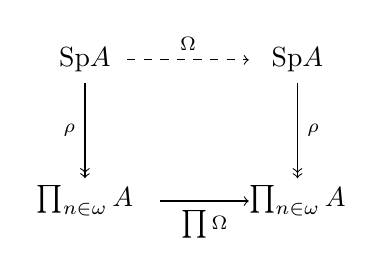
\begin{tikzpicture}[x=1.6em,y=1.5em]
  \node (TL) at (0,1.7) {$\mathrm{Sp}A$};
  \node (TR) at (4.8,1.7) {$\mathrm{Sp}A$};
  \node (BL) at (0,-1.7) {$\prod_{n\in\omega}A$};
  \node (BR) at (4.8,-1.7) {$\prod_{n\in\omega}A$};
  \draw[->,dashed] (0.95,1.7) -- node[above]{$\scriptstyle\Omega$} (3.7,1.7);
  \draw[->>] (0,1.15) -- node[left]{$\scriptstyle\rho$} (0,-1.15);
  \draw[->>] (4.8,1.15) -- node[right]{$\scriptstyle\rho$} (4.8,-1.15);
  \draw[->] (1.7,-1.7) -- node[below]{$\scriptstyle\prod\Omega$} (3.7,-1.7);
\end{tikzpicture}
\end{center}
由 $\mathrm{Sp}A$ 作为\trFlexibleWeightedLimit{}的\trUniversalProperty{}，我们
可以从加权锥
\begin{center}
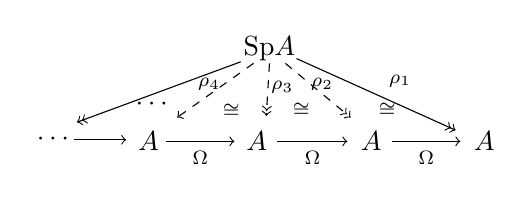
\begin{tikzpicture}[x=1.15em,y=1.15em]
  \node (SpA) at (7.1,3.6) {$\mathrm{Sp}A$};
  \node (dots0) at (0.3,0.75) {$\cdots$};
  \node (A1) at (3.3,0.7) {$A$};
  \node (A2) at (6.7,0.7) {$A$};
  \node (A3) at (10.3,0.7) {$A$};
  \node (A4) at (13.85,0.7) {$A$};
  \node (dots1) at (3.4,1.85) {$\cdots$};
  \draw[->] (0.95,0.75) -- (2.6,0.75);
  \draw[->] (3.85,0.7) -- node[below]{$\scriptstyle\Omega$} (6.0,0.7);
  \draw[->] (7.35,0.7) -- node[below]{$\scriptstyle\Omega$} (9.55,0.7);
  \draw[->] (10.95,0.7) -- node[below]{$\scriptstyle\Omega$} (13.1,0.7);
  \draw[->>] (6.2,3.2) -- (1.05,1.3);
  \draw[->,dashed] (6.6,3.15) -- (4.2,1.45);
  \node at (5.2,2.5) {$\scriptstyle\rho_{4}$};
  \draw[->>,dashed] (7.1,3.15) -- (7.0,1.5);
  \node at (7.5,2.4) {$\scriptstyle\rho_{3}$};
  \draw[->>,dashed] (7.6,3.15) -- (9.65,1.45);
  \node at (8.75,2.5) {$\scriptstyle\rho_{2}$};
  \draw[->>] (7.95,3.3) -- (12.95,1.05);
  \node at (11.2,2.6) {$\scriptstyle\rho_{1}$};
  \node at (5.9,1.65) {$\scriptstyle\cong$};
  \node at (8.1,1.7) {$\scriptstyle\cong$};
  \node at (10.8,1.7) {$\scriptstyle\cong$};
\end{tikzpicture}
\end{center}
——它由沿包含 $\Sigma\colon n\mapsto n+1\colon\omega^{\mathrm{op}}\to\omega^{\mathrm{op}}$
作限制以移位加权极限锥中的数据而得——诱导出另一个自函子
$\Sigma^{*}\colon\mathrm{Sp}A\to\mathrm{Sp}A$。为更形式化地分析这个函子，考虑
自然同构 $\sigma\colon W^{\leftarrow}\cong W^{\leftarrow}\Sigma$ 穿过左%
\trKanExtension{}的因子分解：
\begin{center}
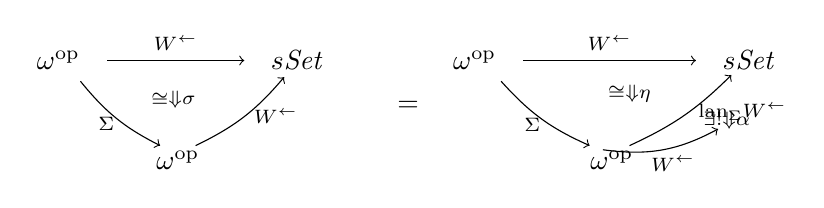
\begin{tikzpicture}[x=1.6em,y=1.5em]
  \begin{scope}[shift={(0,0)}]
  \node (w1) at (0,1.1) {$\omega^{\mathrm{op}}$};
  \node (s1) at (5.4,1.1) {$s\mathit{Set}$};
  \node (b1) at (2.7,-1.3) {$\omega^{\mathrm{op}}$};
  \draw[->] (1.1,1.1) -- node[above]{$\scriptstyle W^{\leftarrow}$} (4.2,1.1);
  \draw[->] (0.5,0.6) to[bend right=12] node[left,pos=0.6]{$\scriptstyle\Sigma$} (2.3,-0.95);
  \draw[->] (3.1,-0.95) to[bend right=12] node[right,pos=0.5]{$\scriptstyle W^{\leftarrow}$} (5.1,0.7);
  \node at (2.6,0.15) {$\scriptstyle\cong\Downarrow\sigma$};
  \end{scope}
  \node at (7.9,0) {$=$};
  \begin{scope}[shift={(9.4,0)}]
  \node (w2) at (0,1.1) {$\omega^{\mathrm{op}}$};
  \node (s2) at (6.2,1.1) {$s\mathit{Set}$};
  \node (b2) at (3.1,-1.3) {$\omega^{\mathrm{op}}$};
  \draw[->] (1.1,1.1) -- node[above]{$\scriptstyle W^{\leftarrow}$} (5.0,1.1);
  \draw[->] (0.6,0.6) to[bend right=12] node[left,pos=0.6]{$\scriptstyle\Sigma$} (2.6,-0.95);
  \draw[->] (3.5,-0.95) to[bend right=10] node[right,pos=0.55]{$\scriptstyle\mathrm{lan}_{\Sigma}W^{\leftarrow}$} (5.8,0.75);
  \draw[->] (2.9,-1.05) to[bend right=18] node[below,pos=0.6]{$\scriptstyle W^{\leftarrow}$} (5.5,-0.55);
  \node at (3.5,0.3) {$\scriptstyle\cong\Downarrow\eta$};
  \node at (5.7,-0.35) {$\scriptstyle\exists!\Downarrow\alpha$};
  \end{scope}
\end{tikzpicture}
\end{center}
如此，映射 $\Sigma^{*}$ 便得以进入加权极限上诱导映射的一张交换图表
\begin{center}
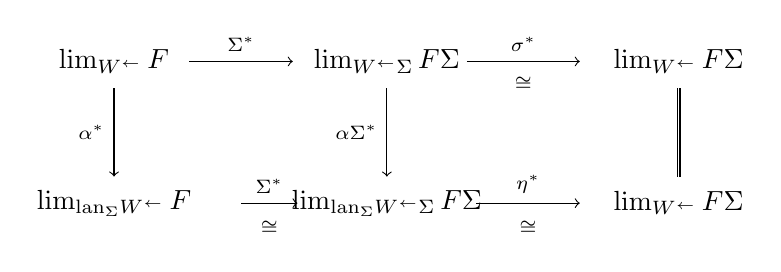
\begin{tikzpicture}[x=1.7em,y=1.6em]
  \node (A1) at (0,1.6) {$\lim_{W^{\leftarrow}}F$};
  \node (A2) at (5.8,1.6) {$\lim_{W^{\leftarrow}\Sigma}F\Sigma$};
  \node (A3) at (12.0,1.6) {$\lim_{W^{\leftarrow}}F\Sigma$};
  \node (B1) at (0,-1.6) {$\lim_{\mathrm{lan}_{\Sigma}W^{\leftarrow}}F$};
  \node (B2) at (5.8,-1.6) {$\lim_{\mathrm{lan}_{\Sigma}W^{\leftarrow}\Sigma}F\Sigma$};
  \node (B3) at (12.0,-1.6) {$\lim_{W^{\leftarrow}}F\Sigma$};
  \draw[->] (1.6,1.6) -- node[above]{$\scriptstyle\Sigma^{*}$} (3.8,1.6);
  \draw[->] (7.5,1.6) -- node[above]{$\scriptstyle\sigma^{*}$} (9.9,1.6);
  \node at (8.7,1.1) {$\scriptstyle\cong$};
  \draw[->] (0,1.0) -- node[left]{$\scriptstyle\alpha^{*}$} (0,-1.0);
  \draw[->] (5.8,1.0) -- node[left]{$\scriptstyle\alpha\Sigma^{*}$} (5.8,-1.0);
  \draw[double] (12.0,1.0) -- (12.0,-1.0);
  \draw[->] (2.7,-1.6) -- node[above]{$\scriptstyle\Sigma^{*}$} (3.9,-1.6);
  \node at (3.3,-2.15) {$\scriptstyle\cong$};
  \draw[->] (7.7,-1.6) -- node[above]{$\scriptstyle\eta^{*}$} (9.9,-1.6);
  \node at (8.8,-2.15) {$\scriptstyle\cong$};
\end{tikzpicture}
\end{center}
注意底行复合展示出引理 A.6.19 的那个同构——这是富集范畴论的一条一般结果，它
说受限制图表的加权极限与以权之左\trKanExtension{}加权的极限相合（见 [68,
4.63]）。由这个结果以及同构 $\sigma\colon W^{\leftarrow}\cong W^{\leftarrow}\Sigma$
与 $F\cong F\Sigma$，我们见到图表中的一切对象都同构于 $\mathrm{Sp}A$。

由于 $\Sigma$ 是\trFullyFaithful{}，$\eta$ 是一个同构，从而 $\alpha\Sigma$
亦然；于是我们所关心的映射 $\Sigma^{*}\colon\mathrm{Sp}A\to\mathrm{Sp}A$ 同构
于由包含 $\alpha\colon\mathrm{lan}_{\Sigma}W^{\leftarrow}\hookrightarrow W^{\leftarrow}$
在加权极限上诱导的映射。这个映射是柔性权之间的一个射影胞腔复形，其定义方式为
在 $0$ 处附接单个广义射影胞腔
$\qcOne\times\omega(-,0)\hookrightarrow\hciso\times\omega(-,0)$。换言之，它在
除一个分量之外的一切分量上都是同构；经由同构
$W^{\leftarrow}\cong\mathrm{lan}_{\Sigma}W^{\leftarrow}\Sigma$，其第零分量为
$\alpha_{0}\colon W^{\leftarrow}_{1}\hookrightarrow W^{\leftarrow}_{0}$。于是
我们见到 $\alpha$ 定义射影胞腔复形之间的一个逐点 Joyal 弱\trEquivalence{}。由%
\trPullback{}图表
\begin{center}
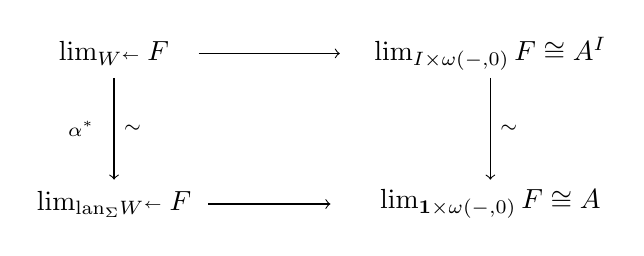
\begin{tikzpicture}[x=1.7em,y=1.6em]
  \node (TL) at (0,1.7) {$\lim_{W^{\leftarrow}}F$};
  \node (TR) at (8.0,1.7) {$\lim_{\hciso\times\omega(-,0)}F\cong A^{\hciso}$};
  \node (BL) at (0,-1.7) {$\lim_{\mathrm{lan}_{\Sigma}W^{\leftarrow}}F$};
  \node (BR) at (8.0,-1.7) {$\lim_{\qcOne\times\omega(-,0)}F\cong A$};
  \draw[->] (1.8,1.7) -- (4.8,1.7);
  \draw[->] (0,1.15) -- node[right]{$\scriptstyle\sim$} (0,-1.15);
  \node at (0.5,0.6) {$\scriptstyle\lrcorner$};
  \node at (-0.7,0) {$\scriptstyle\alpha^{*}$};
  \draw[->] (8.0,1.15) -- node[right]{$\scriptstyle\sim$} (8.0,-1.15);
  \draw[->] (2.0,-1.7) -- (4.6,-1.7);
\end{tikzpicture}
\end{center}
可知加权极限上诱导的映射 $\Sigma^{*}\colon\mathrm{Sp}A\to\mathrm{Sp}A$ 是一个%
\trEquivalence{}。

由构造，复合 $\Omega\Sigma^{*}\colon\mathrm{Sp}A\to\mathrm{Sp}A$ 自然同构于
恒同函子，其中这个同构可以由加权极限锥的同构 $\Omega\rho_{n+1}\cong\rho_{n}$
出发、借助\trPullback{} \eqref{eq:spa-iso-tower} 的弱\trUniversalProperty{}诱导出来。
于是，由\trTwoOfThreeProperty{}以及等价在自然同构下的稳定性，$\Omega$ 是一个%
\trEquivalence{}。

我们已经证明：$\mathrm{Sp}A$ 是一个容有\trPullback{}的带点∞-范畴，其\trLoops{}函子是一个%
\trEquivalence{}。由定理 4.4.12(v)，$\mathrm{Sp}A$ 如所断言是一个\trStable{}
\trInfinityCategory{}。
\end{proof}

\subsection*{练习}

\begin{exercise}\label{ex:replete-local-isofibration}
设 $\mathcal{L}\hookrightarrow\mathcal{K}$ 是某个∞-宇宙的一个充盈子范畴。试
证明：对所有 $A,B\in\mathcal{L}$，映射
\[
\Fun_{\mathcal{L}}(A,B)\hookrightarrow\Fun_{\mathcal{K}}(A,B)
\]
既是\trQuasiCategory{}之间的一个\trMonomorphism{}，又是一个\trIsofibration{}。
后一性质可以概括为：单纯函子 $\mathcal{L}\hookrightarrow\mathcal{K}$ 是一个
\emph{局部等价纤维化}（local isofibration）。\footnote{充盈子范畴的包含在适
用于 $(\infty,2)$-范畴论的意义下亦是\emph{整体等价纤维化}（global
isofibration），即：$\mathcal{K}$ 中涉及子范畴 $\mathcal{L}$ 内一个对象的%
\trEquivalence{}的全部数据均可提升到 $\mathcal{L}$ 中。}
\end{exercise}

\begin{exercise}\label{ex:pointed-comparison}
对任何∞-宇宙 $\mathcal{K}$，试比较\cref{prop:pointed-cosmos}前后讨论中出现的
宇宙论嵌入∞-宇宙 $\mathcal{K}_{\perp}\cap\mathcal{K}_{\top}$ 与
$\mathcal{K}_{*}:=(\mathcal{K}_{\top})_{\perp}\cong(\mathcal{K}_{\perp})_{\top}$。
\end{exercise}

\begin{exercise}\label{ex:lari-codual}
试证明 $\mathcal{L}ari(\mathcal{K})\cong\mathcal{R}ari(\mathcal{K}^{co})^{co}$。
\end{exercise}

\begin{exercise}\label{ex:discrete-cart}
对一个\trCosmologicalEmbedding{}的∞-宇宙 $\mathcal{L}\hookrightarrow\mathcal{K}$，
试证明：$A\in\mathcal{L}$ 是\trDiscrete{}，当且仅当 $A$ 作为 $\mathcal{K}$
的对象是\trDiscrete{}。
\end{exercise}

\begin{exercise}\label{ex:cocartesian-pullback}
（[46, 4.1.5]）给定一张图表，其中诸竖直映射是\trCocartesianFibration{}且诸方块定义笛卡尔
函子
\begin{center}
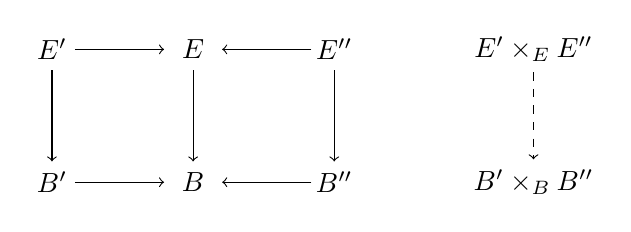
\begin{tikzpicture}[x=1.5em,y=1.5em]
  \node (Ep) at (0,1.6) {$E'$};
  \node (E)  at (3.4,1.6) {$E$};
  \node (Epp) at (6.8,1.6) {$E''$};
  \node (Bp) at (0,-1.6) {$B'$};
  \node (B)  at (3.4,-1.6) {$B$};
  \node (Bpp) at (6.8,-1.6) {$B''$};
  \draw[->] (0.55,1.6) -- (2.7,1.6);
  \draw[->] (6.25,1.6) -- (4.1,1.6);
  \draw[->] (0,1.1) -- (0,-1.1);
  \draw[->] (3.4,1.1) -- (3.4,-1.1);
  \draw[->] (6.8,1.1) -- (6.8,-1.1);
  \draw[->] (0.55,-1.6) -- (2.7,-1.6);
  \draw[->] (6.25,-1.6) -- (4.1,-1.6);
  \node (PE) at (11.6,1.6) {$E'\times_{E}E''$};
  \node (PB) at (11.6,-1.6) {$B'\times_{B}B''$};
  \draw[->,dashed] (11.6,1.05) -- (11.6,-1.05);
\end{tikzpicture}
\end{center}
试验证：诸\trPullback{}之间诱导的函子是一个\trCocartesianFibration{}，且诸投影定义\trCartesianFunctor。
并证明：若诸竖直映射是离散\trCocartesianFibration{}，则这个诱导函子亦然。
\end{exercise}
